% §3 The isotropic theory --- blueprint chapter 3 (blueprint/src/parts/03-isotropic.tex). Written
% from the draft's §3 (Q-0285, 2026-10-04), revised after the blind review
% records/affine/REVIEW-paper-sections-2-3.md (Q-0286, the same day): the blueprint flags were fixed
% at the source and the ten changed statements re-transcribed (records/affine/
% transcribe-shared-statements.py), then the paper-side flags were worked; each flag is answered in
% the review record. Every statement is transcribed verbatim from its node under a
% `% shared with blueprint` marker, with the paper statement's \label equal to the blueprint label,
% so that `linkage check` reports it `verbatim`; only the title of def:isotropic-kernel-family
% differs (titles are not compared).
%
% Order. The draft's, not the blueprint's: the axioms and the reduction to the line first (3.1,
% 3.2), then the origin (3.3) and the filtration (3.4). The blueprint puts the origin and the
% filtration first because the classification names their vocabulary; here the vocabulary is
% introduced where the classification needs it (A_d is section 2's, the origin datum comes before
% prop:isotropic-polar-reading), and the one forward reference that remains is to
% def:filtration-thresholds, which defines A_d again with the witness family.
%
% Proofs. The proofs of record are the blueprint's. Short ones are transcribed; long ones are
% shortened to their decisive steps and headed "Sketch", which section 1.1 explains (Paper V's
% convention: the full proof is in the deposited blueprint sources). After section 2.6 a cited fact
% is named by its number and its \ref, with no repeated page anchor (the author's delegation,
% review flag 44); before each [A] node one sentence names the facts it rests on (flag 14).
% Comparisons with the line are collected in Remark rem:isotropic-line (flag 20); "what else ports" is folded into
% it (flag 50). The figure is records/affine/fig-thresholds.py's (flag 40).
%
% Shortened into Appendix A (Q-0291, the author's decision of 2026-10-04, as Q-0290 did for
% section 5; records/affine/move-sections-3-4-to-appendices*.py): every statement stays here; the
% proofs moved verbatim, but for their headings, except the necessity half of
% thm:isotropic-classification, which is the reduction to the line. One sentence per subsection says
% where its proofs are and which cited facts it rests on.
%
% Q-0307 (the split at §3 | §4, adr/0001): moved from paper/ into the isotropic paper, the
% statements and proofs unchanged. Three sentences that pointed into the affine paper's sections
% (the axiom scheme, the operator lemma of its Appendix B, its use of the logarithmic exponent) now
% name it as a companion paper in prose, with a TODO(module) comment, as an unreleased module is
% cited (article-kit WRITING.md § 4). thm:isotropic-classification and thm:origin-boundedness-d
% re-transcribed from the blueprint, where they had moved since (an F'(0) = 0 in the uniqueness
% clause; the delay law stated as a hypothesis in clause (3)).
%
% Q-0311 (the blind review records/affine/REVIEW-paper-iso.md; REVIEW-paper-iso-fixes.md), paper
% prose only, no shared statement touched: no proof is a sketch any more (Appendix A has the full
% proofs of record); the reduction sentence kept in 3.2 (and section 1) only (flag 33); the
% necessity proof points to Proposition prop:line-filtration for A_d (flag 20); Sato's Theorem 28.4
% and Lemma 28.5 before the threshold theorem (flag 2); kernels "from scale zero" (flag 24); the
% role of lem:isotropic-exponent-log(2) said (flag 10); the Matern coincidence explained by the
% kernel's density (Fischer et al. (2.24), p. 10; READING-fischer2025variance.md) (flag 9); the
% witness's non-monotone delay profile before its definition (flag 30); the remark on 3/2 - sqrt 2
% moved after its proof in Appendix A (flag 31); the caption names no repository path (flag 13);
% Remark rem:isotropic-line counts three results carried and one added (flag 19); cited facts C1-C4.
%
% Q-0316 (pass 2, the blind register review REVIEW-register-paper-iso.md, section 3 flags; answered
% in REVIEW-register-paper-iso-fixes.md), paper prose only but for two NEW shared statements, the
% blueprint's prop:isotropic-radial-monotone (Wolfe's theorem, the cited fact C5, made a statement;
% section 3 flag 1, section 4 flags 1, 3, 15) and lem:delay-polar-profile (the witness's membership,
% Appendix A flag 1), transcribed by records/affine/transcribe-shared-statements.py. The statement-
% zone flags 5, 6, 20, 21, 22 are owed at the blueprint (GATE-paper-iso.md).
%
% Q-0328: a new shared statement, prop:origin-lower-bound-d (Q-0272, refereed blind, sound), in 3.3
% after thm:origin-boundedness-d, transcribed by records/affine/transcribe-q0328-origin-lower-bound.py
% (verbatim); the paragraph that said pointwise bounds were open now leads into it, and the comments
% after it compare it with clause (4). Its proof is in Appendix A.
%
% Q-0334: a new shared statement at the end of 3.1, lem:kernels-to-operators (the blueprint node's
% clauses (1) and (3), rendered and pinned; the comment above it says how). The operator-form
% paragraph claims the converse passage through it, the forward passage still waits on the affine
% paper; Remark rem:isotropic-line names it as the one statement read on operators. Its proof is in
% Appendix A.
%
% Q-0406 (pass 6, the author's review of sections 3.1-3.2; records/affine/
% REVIEW-author-paper-iso.md, "§ 3.1-3.2"). 3.1 opens with the axioms on operators (the new shared
% statement def:isotropic-operator-family), then the kernel form, then ONE lemma for both passages,
% labelled lem:operators-to-kernels here and pinned against the blueprint's lem:operators-to-kernels
% and lem:kernels-to-operators; it replaces the lemma of Q-0334 (label lem:kernels-to-operators,
% gone from this paper), and the forward passage no longer waits on the affine paper. 3.2 is
% introduced for a computer-vision reader (marginal, projection, the plan). The paper's copy of
% lem:isotropic-marginal-family refers to Definition def:line-family and drops the restated list
% (pinned). The polar profile is motivated before def:isotropic-origin-datum. Throughout the
% section, a place of the line paper or the cone paper that section 2 restates is cited at the
% restatement: in shared text through \restated / \restatedp (macros.tex), which the blueprint
% prints as the located citation, so those statements stay verbatim; where a statement or a proof
% also carried a "restated: ..." passage that section 2 gives (prop:isotropic-bridge,
% lem:delay-polar-profile, the necessity half of thm:isotropic-classification), the paper's copy
% drops it and is pinned. Every statement number of the section goes up by one (the new
% Definition 3.1). NOT done, and owed once Q-0381 is merged: the statement of
% def:filtration-thresholds, which Q-0381 rewords on another branch on the very lines that cite
% [B, Prop. 4.9], [B, Def. 4.1], [V, (2.3)] and [B, Def. 4.11] (all four restated in section 2), and
% the proof of thm:filtration-strict in Appendix A ([B, Prop. 4.9(1)] and (4), which are
% Proposition prop:line-filtration(1) and (3)). They keep \prog, the located citation.
%
% Q-0407 (the author's decision on pull request #100): the classification on operators, which
% Q-0406 said in two sentences after the theorem, is a new shared statement,
% cor:isotropic-classification-operators, printed as a corollary after
% thm:isotropic-classification with its proof (the comment above it says how the proof differs from
% the proof of record). Every later statement number of the section goes up by one.
% Remark rem:isotropic-line says what the corollary is at d = 1.
%
% Q-0408 (pass 6, the author's review of sections 3.3 and 3.4: "very technical", "not completely
% sure why the results are interesting", "a bit more guiding to the main results in the
% beginning"; records/affine/REVIEW-author-paper-iso.md). Prose only, and the ORDER of the
% statements in 3.3 and 3.4: each subsection opens with the question, why a vision reader cares
% and the results by number, and its main theorem is stated before the lemmas of its proof. No
% shared statement and no proof is changed; records/affine/edits_q0408_sections.py cuts the
% statements out as they stand and pastes them into the new prose. The statement numbers 3.13 to
% 3.23 change (the table in the review record). The comments at the head of 3.3 and of 3.4 say
% what each opening holds and what it was checked against.
% Second round, the same item (the blind register review of the new prose, 34 flags, answered in
% records/affine/REVIEW-register-paper-iso-q0408-fixes.md; records/affine/edits_q0408_round2.py):
% prose of 3.3 and 3.4 again, no statement changed or moved. One decision of that round reverses
% a line of this header ("before each [A] node one sentence names the facts it rests on", flag 14
% of Q-0286): the body no longer says which cited facts a statement rests on. The cited facts are
% the numbered theorems of section 2.6, and section 1.1 owns the accounting (WRITING.md section
% 3; the dispatching session's decision of 2026-10-10). Sections 3.1 and 3.2 had no such sentence
% left; the one that names C2 before the polar form of A_d says which theorem the proposition
% reads, with Sato's attribution, and stays.
%
% Q-0428 (the rewrite after the external review, round 1; records/affine/
% REPOSITIONING-paper-iso-round2.md). Sections 3.3 and 3.4 are rewritten around the eight
% blueprint nodes of Q-0425, three of which are printed here (prop:origin-rate-profile-d,
% prop:radial-dictionary, cor:dictionary-filtration) and five in Appendix A; the comments at the
% head of the two subsections say how. Statements and proofs of the eight are written by
% records/affine/transcribe-q0428-nodes.py. The statements of prop:origin-lower-bound-d and
% prop:origin-upper-bound-d are in Appendix A since this item, for the length of the main text,
% with a paragraph in 3.3 that says what they give. The statement numbers from 3.16 on changed
% (paper-iso/README.md has the list). In 3.2: the plan names the three parts of the subsection,
% and the Levy density f_d is set against the density p of the kernel (the presentation review
% of round 1, items 13 and 6). def:filtration-thresholds is a pinned copy that takes the classes
% from section 2.

\section{The isotropic theory}\label{sec:isotropic}

% Q-0310 (review flag 12): the section opens on its own terms, with no reference to an axiom scheme
% of groups and orders, which is the affine paper's; the kernels-only disclaimer is said once, after
% Definition def:isotropic-kernel-family (flag 31); "profile" is qualified throughout, the
% contraction ratio of self-decomposability is lambda (records/affine/
% REVIEW-paper-whole-fixes-paper-iso.md); the comparison with Schoenberg has one home, section 1.
% Q-0414, round 2 (the register review of 2026-10-11 on sections 2 and 3, answered in
% REVIEW-register-paper-iso-2026-10-11-fixes.md): the opening names what decides boundedness (the
% number c against d), not "it"; in 3.1 the two forms of the axioms are said to be for different
% uses, the pairing of the axioms is said once, with (ND), and the comparison at d = 1 is left to
% Remark rem:isotropic-line; in 3.2 the lead says which proofs are in the body, the kernel "from
% scale zero to the scale t_1 with chi(t_1) = 1" replaces "at canonical scale 1", the paragraph
% before Lemma lem:isotropic-realisation says what the lemma adds to the theorem's "if" half, the
% comment after Proposition prop:isotropic-polar-reading says what clauses (1) and (3) are for and
% gives one datum, the lead of Proposition prop:isotropic-bridge says what it adds to Proposition
% prop:line-filtration(2); Lemma lem:polar-decomposition and the proof of Corollary
% cor:isotropic-classification-operators are in Appendix A (records/affine/
% edits_q0414_round2_moves.py); "corner" is replaced in prose and in the paper's title of
% Proposition prop:isotropic-bridge (the clause titles inside its shared statement kept it until
% Q-0417, which changed them at the blueprint).
An isotropic family measures a signal on $\RR^d$ through rotation-invariant kernels, and a
dilation of the signal only relabels the scales. This section states the axioms
(\S\ref{sec:isotropic-axioms}), classifies the families by reduction to the line
(\S\ref{sec:isotropic-reduction}), describes a kernel at its centre
(\S\ref{sec:isotropic-origin}) and says how the dimension restricts the exponents
(\S\ref{sec:isotropic-filtration}).

\subsection{The axioms}\label{sec:isotropic-axioms}

% Q-0406 (the author's review of section 3, comment 1): the subsection opens with the axioms on
% operators, as the line papers do (the new shared statement def:isotropic-operator-family, a
% blueprint node since this item), then the kernel form, then one lemma connecting the two in both
% directions. The inline paragraph on the operator form is gone.
The axioms are those of the line, Definition~\ref{def:line-family}, with $\RR^d$ in place of $\RR$
and the orthogonal group in place of the reflection. They are stated on operators, which assumes
neither a convolution nor a probability kernel, and on kernels, which is the form the proofs use.
Lemma~\ref{lem:operators-to-kernels} joins the two. The operator $\Phi_{s,t}$ takes the record of
an image at scale $s$ to its record at the coarser scale $t$.

% shared with blueprint def:isotropic-operator-family
\begin{definition}[isotropic cascade measurement family]\label{def:isotropic-operator-family}
Fix an integer $d \ge 1$. On the real space $L^1(\RR^d)$ write $T_af := f(\cdot - a)$ for the
translation by $a \in \RR^d$, $R_Qf := f(Q^{-1}\,\cdot)$ for the action of an orthogonal matrix
$Q \in \Orth(d)$, and $D_\lambda f := \lambda^{-d}f(\cdot/\lambda)$ for the dilation by
$\lambda > 0$. A family $(\Phi_{s,t})_{0 \le s \le t}$ of linear operators on $L^1(\RR^d)$ is an
\emph{isotropic cascade measurement family in dimension $d$} if:
\begin{enumerate}
\item[(A1)] each $\Phi_{s,t}$ is a bounded operator on $L^1(\RR^d)$;
\item[(A2)] \emph{(translation invariance)} $\Phi_{s,t}T_a = T_a\Phi_{s,t}$ for every
$a \in \RR^d$;
\item[(A3)] \emph{(rotation invariance)} $\Phi_{s,t}R_Q = R_Q\Phi_{s,t}$ for every
$Q \in \Orth(d)$;
\item[(A4)] \emph{(positivity)} $\Phi_{s,t}$ maps nonnegative functions to nonnegative functions;
\item[(A5)] \emph{(mass)} $\int\Phi_{s,t}f = \int f$ for every nonnegative $f \in L^1(\RR^d)$;
\item[(A6)] \emph{(cascade)} $\Phi_{t,t} = \mathrm{Id}$, and $\Phi_{s,t}\Phi_{r,s} = \Phi_{r,t}$
whenever $r \le s \le t$;
\item[(A7)] \emph{(continuity)} for every $f \in L^1(\RR^d)$ the map $(s,t) \mapsto \Phi_{s,t}f$
is continuous from $\{0 \le s \le t\}$ to $L^1(\RR^d)$;
\item[(A8)] \emph{(dilation covariance)} there is a family $(S_\lambda)_{\lambda > 0}$ of
increasing bijections of $[0,\infty)$ with
$D_\lambda\Phi_{s,t} = \Phi_{S_\lambda s,\,S_\lambda t}D_\lambda$ for all $0 \le s \le t$ and all
$\lambda > 0$;
\item[(ND)] \emph{(nondegeneracy)} $\Phi_{s,t} \ne \mathrm{Id}$ whenever $s < t$.
\end{enumerate}
\end{definition}

The numbering is that of the line, and Remark~\ref{rem:isotropic-line} compares the two at $d = 1$.
Axioms (A2) and (A3) say that the measurement prefers no position and no direction. The comments
on (A6), (A8) and (ND) in \S\ref{sec:line-axioms} apply unchanged. By (A1), (A2), (A4) and (A5)
each $\Phi_{s,t}$ is convolution by a probability measure, its \emph{kernel}
(Lemma~\ref{lem:operators-to-kernels}(1) below). The remaining axioms then become conditions on
the kernels.

% shared with blueprint def:isotropic-kernel-family
\begin{definition}[isotropic cascade family]\label{def:isotropic-kernel-family}
Fix an integer $d \ge 1$. For $A \in \GL(d)$ write $A_*\mu := \mu \circ A^{-1}$ for the image of a
measure $\mu$ on $\RR^d$, and $\widehat\mu(\xi) = \int e^{i\langle\xi,x\rangle}\mu(dx)$, so that
$\widehat{A_*\mu}(\xi) = \widehat\mu(A^{\tp}\xi)$. An \emph{isotropic cascade family in dimension
$d$} is a family $(\mu_{s,t})_{0 \le s \le t}$ of probability measures on $\RR^d$ such that
\begin{enumerate}
\item[(I1)] \emph{(cascade)} $\mu_{t,t} = \delta_0$, and $\mu_{r,t} = \mu_{s,t} * \mu_{r,s}$
whenever $r \le s \le t$;
\item[(I2)] \emph{(continuity)} for every $\xi \in \RR^d$ the map
$(s,t) \mapsto \widehat\mu_{s,t}(\xi)$ is continuous on $\{0 \le s \le t\}$;
\item[(I3)] \emph{(rotation invariance)} $Q_*\mu_{s,t} = \mu_{s,t}$ for every $Q \in \Orth(d)$
and every pair;
\item[(I4)] \emph{(dilation covariance)} there is a family $(S_\lambda)_{\lambda > 0}$ of
increasing bijections of $[0,\infty)$ with $(\lambda I)_*\mu_{s,t} = \mu_{S_\lambda s,\,S_\lambda t}$
for every $\lambda > 0$ and every pair;
\item[(ND)] \emph{(nondegeneracy)} $\mu_{s,t} \ne \delta_0$ whenever $s < t$.
\end{enumerate}
\end{definition}

% Q-0406: the paragraph that described the operator form inline, with its TODO(module affine), is
% replaced by Definition def:isotropic-operator-family above and the lemma below. The sentence on
% the vocabulary of section 2 is kept.
The two definitions correspond axiom by axiom. (I1) is the cascade (A6), (I2) the continuity (A7),
(I3) the rotation invariance (A3), (I4) the dilation covariance (A8) with the same bijections
$S_\lambda$, and (ND) is (ND). The next lemma says that the two definitions describe the same
families. The point that needs an argument is its clause (2), that the two continuities are the
same: (A7) requires convergence in $L^1(\RR^d)$, and (I2) convergence of the transforms at
each frequency. The proof is in \suppl{} (\S\ref{supp:proofs-axioms}).

% Q-0406: one lemma for both passages, this paper's own instance of two blueprint nodes of
% chapter 4, rendered and so pinned against both (`linkage check --pin-shared`). It replaces the
% lemma of Q-0334, which had the passage from kernels to operators only. What is taken from where:
%   (1) lem:operators-to-kernels(1), without its strong form of uniqueness (mu * gamma = nu * gamma
%       implies mu = nu), which the proof states and uses;
%   (2) "only if" is lem:kernels-to-operators(1); "if" is lem:operators-to-kernels(3), read at
%       f = gamma (the clause's hypothesis, convergence for every f, is more than that node needs);
%   (3) lem:operators-to-kernels(5), which is lem:operators-to-kernels-families(5), its list of
%       axioms replaced by the reference to Definition def:isotropic-operator-family, whose items
%       are that list. "With the bijections of (A8) in (I4)" is not in the node's statement: its
%       proof of record gives it ((I4) is derived with the S_lambda of (A8)), and the Lean states it
%       (operators_to_kernels_isotropic returns IsIsotropicCascadeFamily mu S for the same S);
%   (4) lem:kernels-to-operators(3), its "satisfy the axioms of lem:operators-to-kernels(5)" said
%       as "form an isotropic cascade measurement family".
% Not taken: the transport clause lem:operators-to-kernels(2), which is in the proof, and the
% clauses on the (G, W) families, which are the affine paper's. The notation T_a, R_Q, D_lambda is
% that of Definition def:isotropic-operator-family.
% Q-0417: in clause (2) the frequency on R^d is xi, the letter of this paper (section 2.1 and the
% notation table), where the blueprint nodes and the affine paper's copy write omega. This copy
% only. Q-0327 then renamed the Gaussian density of the two nodes to varphi; the statement here
% does not name it, the proof in Appendix A follows, and the pins below are those of the nodes as
% Q-0327 left them.
% shared with blueprint lem:operators-to-kernels@2a7e1cea1dd4+64892e862e28, lem:kernels-to-operators@8416f2c7edd3+97e85f9d59a2
\begin{lemma}[operators and kernels in dimension $d$]\label{lem:operators-to-kernels}
Fix $d \ge 1$, and for a probability measure $\mu$ on $\RR^d$ and $f \in L^1(\RR^d)$ write
$(\mu * f)(x) := \int f(x - y)\,\mu(dy)$.
\begin{enumerate}
\item \emph{(One operator.)} Let $\Phi$ be a linear operator on $L^1(\RR^d)$ with the four axioms
of Definition~\ref{def:isotropic-operator-family} that concern one operator: (A1) $\Phi$ is
bounded; (A2) $\Phi T_a = T_a\Phi$ for every $a \in \RR^d$; (A4) $\Phi f \ge 0$ whenever
$f \ge 0$; (A5) $\int\Phi f = \int f$ whenever $f \ge 0$. Then there is a unique probability
measure $\mu$ on $\RR^d$ with
\[
  \Phi f = \mu * f, \qquad f \in L^1(\RR^d) .
\]
Conversely, for every probability measure $\mu$ on $\RR^d$ the operator $f \mapsto \mu * f$
satisfies (A1), (A2), (A4) and (A5).
\item \emph{(Continuity.)} Let $\mu_n$ and $\mu$ be probability measures on $\RR^d$. Then
$\widehat\mu_n(\xi) \to \widehat\mu(\xi)$ for every $\xi \in \RR^d$ if and only if
$\mu_n * f \to \mu * f$ in $L^1(\RR^d)$ for every $f \in L^1(\RR^d)$.
\item \emph{(From operators to kernels.)} Let $(\Phi_{s,t})_{0 \le s \le t}$ be an isotropic
cascade measurement family in dimension $d$ (Definition~\ref{def:isotropic-operator-family}), and
for each pair let $\mu_{s,t}$ be the probability measure that (1) gives for $\Phi_{s,t}$. Then
$(\mu_{s,t})_{0 \le s \le t}$ is an isotropic cascade family in dimension $d$
(Definition~\ref{def:isotropic-kernel-family}), with the bijections $S_\lambda$ of (A8) in (I4).
\item \emph{(From kernels to operators.)} Let $(\mu_{s,t})_{0 \le s \le t}$ be an isotropic cascade
family in dimension $d$. Then the operators $\Phi_{s,t}f := \mu_{s,t} * f$ on $L^1(\RR^d)$ form an
isotropic cascade measurement family in dimension $d$, with the bijections $S_\lambda$ of (I4) in
(A8), and the probability measure that (1) gives for $\Phi_{s,t}$ is $\mu_{s,t}$.
\end{enumerate}
\end{lemma}

Clause (1) is Lemma~\ref{lem:line-representation} in $\RR^d$, without the reflection. Clauses (3)
and (4) are inverse to each other: the operators that (4) builds from the kernels of (3) are the
$\Phi_{s,t}$, and the last assertion of (4) says that (3) returns the kernels. So convolution is a
one-to-one correspondence between the isotropic cascade families and the isotropic cascade
measurement families in dimension $d$. From here on a family on $\RR^d$ is given by its kernels.

\subsection{Reduction to the line}\label{sec:isotropic-reduction}

% Q-0406 (the author's review of section 3, comment 2): the subsection is introduced for a
% computer-vision reader: what a marginal is (a projection, as in tomography), why a
% rotation-invariant kernel has one marginal, why it determines the kernel, and the plan.
This subsection classifies the isotropic families by reducing them to the line. The tool is the
projection of a kernel on a line through the origin. Fix a unit vector $e \in \RR^d$. The
\emph{marginal} of a law $\mu$ on $\RR^d$ along $e$ is its image under
$x \mapsto \langle e, x\rangle$, a law on $\RR$. If $\mu$ has a density $p$ and $d \ge 2$, the
marginal has the density
\[
  y \;\longmapsto\; \int_{e^\perp} p(ye + z)\,dz , \qquad y \in \RR ,
\]
the integral of $p$ over the hyperplane through $ye$ orthogonal to $e$. In the plane these are the
integrals of $p$ along the lines orthogonal to $e$. This is the projection of tomography: taken
along every direction, the marginals are the Radon transform of $p$
(\sscite{natterer2001mathematics}, \S II.1, p.~9).
% The Radon transform and the projection-slice theorem are cited from Natterer, read at the page
% (records/affine/READING-natterer2001mathematics.md). His Theorem 1.1 is for Schwartz functions
% and a unitary transform with the other sign; the sentence below says so, and Lemma
% lem:radial-marginal proves the identity for laws, in this paper's convention.

Two facts make the reduction work. A rotation-invariant kernel has the same marginal along every
line, because a rotation takes any line through the origin to any other and leaves the kernel
unchanged. And this one marginal $\kappa$ determines the kernel. The Fourier transform of a
marginal is the transform of the kernel restricted to the line,
$\widehat\kappa(\omega) = \widehat\mu(\omega e)$, which is the projection-slice theorem of
tomography (\sscite{natterer2001mathematics}, Thm.~II.1.1, p.~11, for smooth rapidly decreasing
densities and with another sign and normalization of the transform). The transform of a rotation-invariant kernel is radial, so its values on one line give
it everywhere: $\widehat\mu(\xi) = \widehat\kappa(|\xi|)$. Lemma~\ref{lem:radial-marginal} states
both facts.

The marginals $\kappa_{s,t}$ of an isotropic family inherit its axioms, because projection takes a
convolution to a convolution and a dilation to a dilation. So they are the kernels of a family on
the line in the sense of Definition~\ref{def:line-family}
(Lemma~\ref{lem:isotropic-marginal-family}). The classification on the line,
Theorem~\ref{thm:line-classification}, gives their transforms, and the identity
$\widehat\mu_{s,t}(\xi) = \widehat\kappa_{s,t}(|\xi|)$ carries the answer back to $\RR^d$
(Theorem~\ref{thm:isotropic-classification}). The subsection has three parts: the classification
by projection, a test for membership in $\mathcal{A}_d$ by the polar profile
(Proposition~\ref{prop:isotropic-polar-reading}), and the Gaussian variance mixtures whose
mixing law is a kernel of a time-causal family, which lie in every class
(Proposition~\ref{prop:isotropic-bridge}). The necessity half of the
classification is proved here, and its other proofs in \S\ref{app:classification-proofs}.
The proofs of Lemma~\ref{lem:isotropic-marginal-family} and of
Proposition~\ref{prop:isotropic-bridge} are in \suppl{} (\S\ref{supp:proofs-reduction}).

% shared with blueprint lem:radial-marginal
\begin{lemma}[a rotation-invariant law is determined by its marginal]\label{lem:radial-marginal}
Let $d \ge 1$, let $e \in \RR^d$ be a unit vector and $\pi(x) := \langle e, x\rangle$, and for a
probability measure $\mu$ on $\RR^d$ write $\pi_*\mu$ for its image on $\RR$.
\begin{enumerate}
\item If $Q_*\mu = \mu$ for every $Q \in \Orth(d)$, then $\kappa := \pi_*\mu$ is a symmetric
probability measure on $\RR$, and
\[
  \widehat\mu(\xi) = \widehat\kappa(|\xi|), \qquad \xi \in \RR^d .
\]
In particular $\widehat\mu$ is real and radial, and $\kappa$ does not depend on $e$.
\item Under the hypothesis of (1), $\pi_*\mu = \delta_0$ if and only if $\mu = \delta_0$.
\item For all probability measures $\mu, \mu'$ on $\RR^d$ and every $\lambda > 0$,
$\pi_*(\mu * \mu') = \pi_*\mu * \pi_*\mu'$, $\pi_*\bigl((\lambda I)_*\mu\bigr) =
(\lambda I)_*(\pi_*\mu)$ on $\RR$, and $\pi_*\delta_0 = \delta_0$.
\end{enumerate}
\end{lemma}

Clause (2) is what carries the nondegeneracy (ND) to the line, in every dimension.

% Q-0406 (the author's review of section 3, comment 3): the paper's copy ends at "with the same
% (S_lambda)". The list (A1)-(A8), (ND) that the blueprint node restates from [V, Def. 3.1] is
% Definition def:line-family of section 2 here, and the reader is sent there. The blueprint keeps
% its list, since it has no section 2. Deliberately edited, and pinned.
% shared with blueprint lem:isotropic-marginal-family@e81ae6e86684+f75ee0c4dd9e
\begin{lemma}[the marginals of an isotropic family form a family on the line]\label{lem:isotropic-marginal-family}
Let $(\mu_{s,t})$ be an isotropic cascade family in dimension $d$ with dilation action
$(S_\lambda)$, let $e$ and $\pi$ be as in Lemma~\ref{lem:radial-marginal}, and put
\[
  \kappa_{s,t} := \pi_*\mu_{s,t}, \qquad \Phi_{s,t}f := \kappa_{s,t} * f
  \quad (f \in L^1(\RR)), \qquad 0 \le s \le t .
\]
Then $\widehat\mu_{s,t}(\xi) = \widehat\kappa_{s,t}(|\xi|)$ for every $\xi \in \RR^d$, each
$\kappa_{s,t}$ is a symmetric probability measure, and $(\Phi_{s,t})$ is a symmetric cascade
measurement family in the sense of \restated{V}{Def.~3.1}{def:line-family}, with the same $(S_\lambda)$.
\end{lemma}

The classification in dimension $d$ is now the line's theorem applied to the marginals. The class
$\mathcal{A}_d$ of Proposition~\ref{prop:line-filtration} comes from the cascade itself: the
kernel from scale zero to the scale $t_1$ with $\chi(t_1) = 1$ is self-decomposable, with the
stages as its residuals. A gauge, self-decomposability \ref{eq:self-decomposable} and the
admissible exponents \ref{eq:admissible-line} are as in \S\ref{sec:line-axioms}.

% shared with blueprint thm:isotropic-classification+ef2af91ffb94
\begin{theorem}[the isotropic classification in dimension $d$]\label{thm:isotropic-classification}
% Q-0281 wave 1 (group E): proved. AffineHemigroup.isotropic_classification prints, besides Lean
% core, this module's own ledger A3, clauses (ii) and (iii) (levy_khintchine_unique,
% levy_khintchine_converse; Sato Thm. 8.1), at d = 1, through line_levy_unique
% (prop:line-levy-unique), and nothing of Paper V's: since Q-0365 the development reads the shared
% library's declarations, and blueprint/trust-boundary.txt has no include line. (Until then it
% printed Paper V's cited interface SpatialLine.fourier_toolbox_levy_unique.) The declaration is
% pinned in CIAxiomGuard.lean. The other two declarations of the tag are guarded there too.
Let $d \ge 1$. A family $(\mu_{s,t})_{0 \le s \le t}$ of probability measures on $\RR^d$ is an
isotropic cascade family in dimension $d$ if and only if there are a gauge $\chi$ and an
$F \in \mathcal{A}_d$ with $F \not\equiv 0$ such that
\begin{equation}\label{eq:isotropic-classification}
  \widehat\mu_{s,t}(\xi) = \exp\bigl[-\bigl(F(\chi(t)|\xi|) - F(\chi(s)|\xi|)\bigr)\bigr],
  \qquad 0 \le s \le t,\ \xi \in \RR^d .
\end{equation}
In particular the kernels from scale zero are $\widehat\mu_{0,t}(\xi) = e^{-F(\chi(t)|\xi|)}$. The
pair is unique up to $(\chi,F) \mapsto (c\,\chi,\,F(c^{-1}\,\cdot))$ with $c > 0$, in the sense that if a gauge $\chi'$
and a real function $F'$ on $[0,\infty)$ with $F'(0) = 0$ also satisfy
\ref{eq:isotropic-classification}, then
$\chi' = c\,\chi$ and $F' = F(c^{-1}\,\cdot)$ for some $c > 0$, and $c = 1$ when
$\chi(1) = \chi'(1) = 1$.
\end{theorem}

% Q-0406 (the author's review of section 3, item 5): the necessity paragraph cites the line's
% theorem and the uniqueness of a kernel at their restatements in section 2
% (Theorem thm:line-classification, Lemma lem:line-representation). The proof of record restates
% the theorem in the form it reads and proves the uniqueness in a parenthesis, since the blueprint
% has no section 2. The steps are the same. Deliberately edited, and pinned, as before.
\begin{proof}
\emph{Necessity.} Let $(\mu_{s,t})$ be an isotropic cascade family and let $\kappa_{s,t}$ and
$\Phi_{s,t}$ be as in Lemma~\ref{lem:isotropic-marginal-family}. By that lemma $(\Phi_{s,t})$ is a
symmetric cascade measurement family in the sense of
\restated{V}{Def.~3.1}{def:line-family}, and it is convolution by the symmetric probability
measures $\kappa_{s,t}$. \restated{V}{Thm.~7.3}{thm:line-classification} gives a gauge $\chi$, an
admissible $F \not\equiv 0$ and probability measures $\nu_{s,t}$ on $\RR$ with
$\Phi_{s,t}f = \nu_{s,t} * f$ and
$\widehat\nu_{s,t}(\omega) = \exp[-(F(\chi(t)\omega) - F(\chi(s)\omega))]$. An operator of the
family has only one kernel (Lemma~\ref{lem:line-representation}), so $\nu_{s,t} = \kappa_{s,t}$.
With $\widehat\mu_{s,t}(\xi) = \widehat\kappa_{s,t}(|\xi|)$ from
Lemma~\ref{lem:isotropic-marginal-family}, this gives \ref{eq:isotropic-classification}.

It remains to see $F \in \mathcal{A}_d$. $F$ is admissible, since it has the form
\ref{eq:admissible-line}, and $F(0) = 0$. Put $t_1 := \chi^{-1}(1)$ and $\mu := \mu_{0,t_1}$, so
that $\widehat\mu(\xi) = e^{-F(|\xi|)}$, because $\chi(0) = 0$. For $\lambda \in (0,1)$ put
$s_\lambda := \chi^{-1}(\lambda) \in (0,t_1)$. By \ref{eq:isotropic-classification},
$\widehat\mu(\lambda\xi) = e^{-F(\lambda|\xi|)}$ and
$\widehat\mu_{s_\lambda,t_1}(\xi) = e^{-(F(|\xi|) - F(\lambda|\xi|))}$, so
\[
  \widehat\mu(\xi) = \widehat\mu(\lambda\xi)\,\widehat\mu_{s_\lambda,t_1}(\xi) ,
\]
which is \ref{eq:self-decomposable} with residual $\rho_\lambda = \mu_{s_\lambda,t_1}$. So $\mu$ is
self-decomposable, $\xi \mapsto F(|\xi|)$ is its exponent, and $F \in \mathcal{A}_d$.
The sufficiency and the uniqueness halves are proved in Appendix~\ref{app:isotropic-proofs}.
\end{proof}

% Q-0407 (the author's decision of 2026-10-10 on pull request #100): the classification on
% operators is a numbered statement, the blueprint node cor:isotropic-classification-operators,
% machine-checked (AffineHemigroup.isotropic_classification_operators and
% isotropic_classification_operators_unique). It replaces the two sentences of Q-0406 that said it
% in prose after the theorem. The statement is verbatim. The proof is the proof of record with the
% lemma's clauses re-pointed to this paper's one Lemma lem:operators-to-kernels (its clause (3) is
% the blueprint's lem:operators-to-kernels(5), its clause (4) the blueprint's
% lem:kernels-to-operators(3)) and without the proof of record's last paragraph on what is
% machine-checked, which section 1.1 carries (as Q-0344 and Q-0377 did for other proofs).
% Deliberately edited, and pinned. The blueprint's environment is `theorem`, since it has no
% `corollary`; the label is the same.
With Lemma~\ref{lem:operators-to-kernels} the theorem classifies the operators as well.

% shared with blueprint cor:isotropic-classification-operators+ddc5914f2791
\begin{corollary}[the isotropic classification on operators]\label{cor:isotropic-classification-operators}
Let $d \ge 1$. A family $(\Phi_{s,t})_{0 \le s \le t}$ of linear operators on $L^1(\RR^d)$ is an
isotropic cascade measurement family in dimension $d$ (Definition~\ref{def:isotropic-operator-family}) if and
only if there are a gauge $\chi$, an $F \in \mathcal{A}_d$ with $F \not\equiv 0$, and probability
measures $\mu_{s,t}$ on $\RR^d$ satisfying \ref{eq:isotropic-classification}, such that
\[
  \Phi_{s,t}f = \mu_{s,t} * f, \qquad 0 \le s \le t,\ f \in L^1(\RR^d) .
\]
The measures are then unique, and the pair is unique up to
$(\chi,F) \mapsto (c\,\chi,\,F(c^{-1}\,\cdot))$ with $c > 0$, in the sense that if a gauge $\chi'$,
a real function $F'$ on $[0,\infty)$ with $F'(0) = 0$, and probability measures $\mu'_{s,t}$ on
$\RR^d$ satisfying \ref{eq:isotropic-classification} with $(\chi', F')$ in place of $(\chi, F)$
also give $\Phi_{s,t}f = \mu'_{s,t} * f$ for all $0 \le s \le t$ and all $f \in L^1(\RR^d)$, then
$\mu'_{s,t} = \mu_{s,t}$ for all $0 \le s \le t$, and $\chi' = c\,\chi$ and
$F' = F(c^{-1}\,\cdot)$ for some $c > 0$, and $c = 1$ when $\chi(1) = \chi'(1) = 1$.
\end{corollary}

The `if' half of the theorem
takes probability measures with the transforms \ref{eq:isotropic-classification} as given. The
next lemma supplies them for every pair $(\chi, F)$, from the residuals of the law with exponent
$F(|\cdot|)$. With the uniqueness clause, the pairs therefore parametrise the isotropic cascade
families, up to the rescaling $(\chi,F) \mapsto (c\,\chi, F(c^{-1}\,\cdot))$.

% shared with blueprint lem:isotropic-realisation+f800c22e6ed8
\begin{lemma}[every pair is realised]\label{lem:isotropic-realisation}
Let $d \ge 1$, let $\chi$ be a gauge, and let $F \in \mathcal{A}_d$ with $F \not\equiv 0$. Then
there is an isotropic cascade family $(\mu_{s,t})_{0 \le s \le t}$ in dimension $d$ that satisfies
\ref{eq:isotropic-classification} with the pair $(\chi, F)$.
\end{lemma}

% Q-0448 (review B, S3, of the second external round; records/affine/NODES-q0434.md, section
% 1): the main result as one statement, the blueprint node cor:isotropic-scale-zero-kernels of
% Q-0434, verbatim (the blueprint's environment is `theorem`, since it has no `corollary`; the
% label is the same). Machine-checked: scale_zero_kernels, scale_zero_operators,
% scale_zero_families, scale_zero_relabelling. Its proof is in section A.2 with the other proofs
% of the classification; it cites Proposition prop:isotropic-polar-reading(2), which is stated
% after it, and no proof below depends on the corollary.
% Q-0448, the blind draft review (flag 25): the lead says the statement; the comment after it
% starts at clause (3), since the corollary's own last sentence reads clause (1), and says
% where the proof is.
The theorem and the lemma give the main result: a law is a kernel from scale zero to a positive
scale of an isotropic family exactly when it is rotation invariant, self-decomposable and not the point
mass at the origin.

% shared with blueprint cor:isotropic-scale-zero-kernels+57584c34031d
\begin{corollary}[the kernels from scale zero are the rotation-invariant self-decomposable laws other than $\delta_0$]\label{cor:isotropic-scale-zero-kernels}
Let $d \ge 1$ and let $\mu$ be a probability measure on $\RR^d$. Consider the condition
\begin{enumerate}
\item[(S)] $\mu$ is rotation invariant, that is $Q_*\mu = \mu$ for every $Q \in \Orth(d)$, it is
self-decomposable, and $\mu \ne \delta_0$.
\end{enumerate}
\begin{enumerate}
\item \emph{(On kernels.)} (S) holds if and only if there are an isotropic cascade family
$(\mu_{s,t})_{0 \le s \le t}$ in dimension $d$ and a scale $t > 0$ with $\mu_{0,t} = \mu$.
\item \emph{(On operators.)} (S) holds if and only if there are an isotropic cascade measurement
family $(\Phi_{s,t})_{0 \le s \le t}$ in dimension $d$ (Definition~\ref{def:isotropic-operator-family}) and
a scale $t > 0$ with $\Phi_{0,t}f = \mu * f$ for every $f \in L^1(\RR^d)$.
\item \emph{(The families with this kernel.)} Suppose (S). Then there is an $F \in \mathcal{A}_d$
with $F \not\equiv 0$ and $\widehat\mu(\xi) = e^{-F(|\xi|)}$ for every $\xi \in \RR^d$, and $\mu$
determines $F$ on $[0,\infty)$. Let $t_1 > 0$. A family $(\mu_{s,t})_{0 \le s \le t}$ of
probability measures on $\RR^d$ is an isotropic cascade family in dimension $d$ with
$\mu_{0,t_1} = \mu$ if and only if it satisfies \ref{eq:isotropic-classification} with this $F$
and a gauge $\chi$ with $\chi(t_1) = 1$. The gauge is then unique. For every gauge $\chi$ with
$\chi(t_1) = 1$ there is exactly one such family, and its kernels from scale zero are the
dilations of $\mu$: $\mu_{0,t} = (\chi(t)I)_*\mu$ for every $t > 0$.
\item \emph{(Up to the relabelling of the scales.)} Let $t_1 > 0$, and let
$(\mu_{s,t})_{0 \le s \le t}$ and $(\mu'_{s,t})_{0 \le s \le t}$ be isotropic cascade families
in dimension $d$ with $\mu'_{0,t_1} = \mu_{0,t_1}$. Then there is an increasing bijection
$\theta$ of $[0,\infty)$ with $\theta(t_1) = t_1$ and
$\mu'_{s,t} = \mu_{\theta(s),\theta(t)}$ for all $0 \le s \le t$. If $\chi$ and $\chi'$ are the
gauges that clause (3) gives the two families, for the law $\mu = \mu_{0,t_1}$, then
$\theta := \chi^{-1} \circ \chi'$ is such a bijection.
\end{enumerate}
So the rotation-invariant self-decomposable laws on $\RR^d$ other than the point mass at the
origin are exactly the kernels from scale zero to a positive scale of the isotropic cascade
families in dimension $d$, and a family with a given kernel from scale zero to a given scale is
determined by the gauge (clause (3)), that is up to the relabelling of the scales (clause (4)).
\end{corollary}

Clause (3) says how a family is
recovered from one of its kernels. The law gives the exponent, and what is left free is the
gauge. By clause (4) two families with the same kernel from scale zero to a positive scale
differ by a relabelling of the scales and by nothing else. The proof is in \S\ref{app:classification-proofs}. It uses the
description of the class $\mathcal{A}_d$ in
Proposition~\ref{prop:isotropic-polar-reading}(2) below.

% Q-0406 (the author's review of section 3, comment 4): why A_d needs an explicit form, and what
% the polar profile is, said before the definition: the k of (2.1) in polar coordinates.
The theorem names the class $\mathcal{A}_d$ and does not say which functions belong to it. The
rest of the subsection gives the members an explicit form. On the line that form is
\ref{eq:admissible-line}: a Gaussian coefficient $a_{\mathrm V}$ and a nonincreasing folded
profile $k$, with $k(x)\,dx/x$ the rate at which displacements of size about $x$ occur. In
$\RR^d$ the same two data appear in polar coordinates.
A rotation-invariant \Levy{} measure $\nu_d$ with a density has a radial one, $f_d(|x|)$. It is
the rate of the displacements per unit volume, not the density of the kernel, which is written
$p$ from \S\ref{sec:isotropic-origin} on. The role of $k$ is played by the \emph{polar profile}
\[
  k_d(r) := |S^{d-1}|\,r^d\,f_d(r) , \qquad r > 0 ,
\]
the radial density times $|S^{d-1}|\,r^d$. The factor is chosen so that the displacements of size
between $r_1$ and $r_2$ have the rate $\nu_d(\{r_1 < |x| < r_2\}) = \int_{r_1}^{r_2} k_d(r)\,dr/r$,
the formula of the line. At $d = 1$ the polar profile is the folded profile $k$ of
\ref{eq:admissible-line}, and the Gaussian coefficients are related by $a = 2a_{\mathrm V}$
(Proposition~\ref{prop:isotropic-polar-reading}(2)). The class $\mathcal{A}_d$ then has the
description of the line: its members are the exponents of the pairs $(a, k_d)$ with $k_d$
nonincreasing (Proposition~\ref{prop:isotropic-polar-reading}). The next definition fixes this
vocabulary. It serves \S\ref{sec:isotropic-origin} as well, where the limit $k_d(0{+})$ of the
polar profile at radius $0$ decides how the kernel behaves at its own centre, the origin of
$\RR^d$. Hence the name \emph{origin datum}.
% "The limit k_d(0+)", not "the polar profile at radius 0": the profile is defined on (0, infty).
% Q-0381 makes the same correction to the paragraph this one replaces, on its own branch.

% shared with blueprint def:isotropic-origin-datum
\begin{definition}[isotropic origin data in dimension $d$, and the polar profile]\label{def:isotropic-origin-datum}
Fix an integer $d \ge 1$ and write $\sigma_{d-1}$ for the surface measure of the unit sphere
$S^{d-1} \subset \RR^d$ and $|S^{d-1}| = \sigma_{d-1}(S^{d-1})$ for its surface area. An
\emph{isotropic origin datum in dimension $d$} is a pair
$(a, k_d)$ with $a \ge 0$ and $k_d : (0,\infty) \to [0,\infty)$ nonincreasing, subject to
\[
  \int_0^1 k_d(r)\,r\,dr < \infty
  \qquad\text{and}\qquad
  \int_1^\infty k_d(r)\,\frac{dr}{r} < \infty .
\]
Its \Levy{} measure is the rotation-invariant measure $\nu_d$ on $\RR^d \setminus \{0\}$ with radial
density $f_d(r) = k_d(r)\,\bigl(|S^{d-1}|\,r^d\bigr)^{-1}$, so that
\begin{equation}\label{eq:polar-decomposition}
  \int_{\RR^d} g \,d\nu_d
   = \frac{1}{|S^{d-1}|}\int_{S^{d-1}}\!\!\sigma_{d-1}(d\eta)\int_0^\infty g(r\eta)\,k_d(r)\,\frac{dr}{r}
\end{equation}
for every nonnegative Borel $g$ vanishing at the origin. Its \emph{exponent} is
\begin{equation}\label{eq:isotropic-exponent}
  F_d(\xi) = \tfrac12 a|\xi|^2
   + \int_{\RR^d}\bigl(1 - \cos\langle \xi, x\rangle\bigr)\,\nu_d(dx), \qquad \xi \in \RR^d ,
\end{equation}
and its \emph{law} is the symmetric infinitely divisible law $\mu$ on $\RR^d$ with
$\widehat\mu = e^{-F_d}$. We call $k_d$ the datum's \emph{polar profile} and
$c := k_d(0{+}) \in [0,\infty]$ its \emph{profile at the origin}. The datum is
\emph{subordinated} when there is a delay datum $(a, k_{\mathrm I})$ in the sense of
\restated{B}{Def.~4.11}{sec:line-bridge}, with $k_{\mathrm I}$ nonincreasing, whose polar profile \prog{B}{(4.6)} is $k_d$:
\begin{equation}\label{eq:polar-profile-d}
  k_d(r) = \frac{2}{\Gamma(d/2)}\int_0^\infty v^{d/2-1}e^{-v}\,
    k_{\mathrm I}\Bigl(\frac{r^2}{2v}\Bigr)\,dv , \qquad r > 0 .
\end{equation}
\end{definition}

The polar profile is the integral over the sphere of the profile $k_\eta$ of the polar
criterion C2 (\S\ref{sec:cited-facts}). The delay datum and its delay profile $k_{\mathrm I}$
are those of \S\ref{sec:line-bridge}, and \ref{eq:polar-profile-d} is how a delay profile
becomes a polar profile. The identity \ref{eq:polar-decomposition} is polar coordinates
(Lemma~\ref{lem:polar-decomposition} in the appendix). The next proposition describes
$\mathcal{A}_d$ in polar form, by that criterion.

% Q-0414, round 2: the attribution of the polar criterion is at C2's statement in section 2.6
% (register flag 27: the lead repeated the anchor against section 2.6's rule).
% shared with blueprint prop:isotropic-polar-reading+a05b6f8669b9
\begin{proposition}[the polar form of $\mathcal{A}_d$]\label{prop:isotropic-polar-reading}
Let $d \ge 1$ and $F : [0,\infty) \to [0,\infty)$.
\begin{enumerate}
\item \emph{(The reading.)} $\xi \mapsto F(|\xi|)$ is the exponent of a self-decomposable law on
$\RR^d$ if and only if it is the exponent $F_d$ of an isotropic origin datum $(a,k_d)$ in
dimension $d$ (Definition~\ref{def:isotropic-origin-datum}):
\[
  F(|\xi|) = \tfrac12 a|\xi|^2 + \int_{\RR^d}\bigl(1 - \cos\langle\xi,x\rangle\bigr)\,
    \frac{k_d(|x|)}{|S^{d-1}|\,|x|^d}\,dx , \qquad \xi \in \RR^d .
\]
The datum is then unique, $k_d$ up to modification on a Lebesgue-null set.
\item \emph{(The class.)} If this holds, $F$ is admissible, of the form
\ref{eq:admissible-line} with $a_{\mathrm V} = \tfrac12 a'$ and $k = k_1$ for its datum
$(a',k_1)$ in dimension $1$. So $\mathcal{A}_d$ is the set of $F$ for which $F(|\cdot|)$ is the
exponent of an isotropic origin datum in dimension $d$.
\item \emph{(The classification in polar form.)} A family $(\mu_{s,t})_{0 \le s \le t}$ of
probability measures on $\RR^d$ is an isotropic cascade family in dimension $d$ if and only if
there are a gauge $\chi$ and an isotropic origin datum $(a,k_d)$ in dimension $d$, not both trivial
($a > 0$, or $k_d$ not almost everywhere $0$), with \ref{eq:isotropic-classification} for
\[
  F(r) = \tfrac12 a\,r^2 + \int_{\RR^d}\bigl(1 - \cos(r\langle e_1,x\rangle)\bigr)\,
    \frac{k_d(|x|)}{|S^{d-1}|\,|x|^d}\,dx , \qquad r \ge 0 .
\]
\end{enumerate}
\end{proposition}

Clause (1) is the test for membership in $\mathcal{A}_d$, and the uniqueness of the datum is what
lets \S\ref{sec:isotropic-origin} speak of the profile at the origin of a kernel. Clause (3) is
the classification with the class written out. For example, the datum
$(0, b\,\mathbf{1}_{(0,\tau)})$ has the \Levy{} density $b\,(|S^{d-1}|\,|x|^d)^{-1}$ on the ball
of radius $\tau$ and none outside it, and its exponent is in $\mathcal{A}_d$. For $d \ge 2$ that
exponent is not a member of a $\Cin$ ray
(Proposition~\ref{prop:profile-one-dimension-down}(3)), although a $\Cin$ ray has the same step
as its folded profile: the polar profile is not the folded profile of the same exponent. One exponent has a
datum in each
dimension that admits it, with a different polar profile in each, and the folded profile belongs
to its marginal.

The bridge from the time-causal theory (\S\ref{sec:line-bridge}) carries over to $\RR^d$. The
variance mixtures of $d$-dimensional Gaussians against the kernels of a time-causal family form
an isotropic family in every dimension. That their exponents lie in every $\mathcal{A}_d$ is
Proposition~\ref{prop:line-filtration}(2). The next proposition adds the kernels themselves, as
explicit mixtures with their gauge, and names three families by their transforms: the \Matern{}
kernels, which are the example of \S\ref{sec:isotropic-origin}, and, recorded for reference, the
stable kernels and the Student-t kernels.

% Q-0406 (the author's review of section 3, item 5): the paper's copy says "causally admissible in
% the sense of Definition def:line-causal" and drops the formula and conditions that the blueprint
% node restates from [B, Def. 4.1] after "restated:", which section 2 gives. The statement names
% neither b_0 nor k_I afterwards. Deliberately edited, and pinned.
% Q-0417: the blueprint node's clause titles say "kernels" for "corner" and its clause (4) "a
% time-causal family as above" for "a causal family as above, the causal Bessel family"; the copy
% below follows and is re-pinned, and the lead above no longer says that the statement calls the
% three families corners.
% Q-0431 (the author's section review of 2026-10-12): clause (4) as reworded at the blueprint
% (records/affine/edits_q0431_blueprint_clause4.py): its title is "The Student-t kernels", and
% "if the inverse-gamma laws are the delay kernels of the family" replaces the parenthesis on
% what the cone paper leaves as a hypothesis. The logical form is the same. Re-pinned, this
% marker alone (records/formalization/pin-one-marker.py). The lead no longer says "under a
% hypothesis".
% shared with blueprint prop:isotropic-bridge@b6e24c6ab78f+30da3ba9bb1b
\begin{proposition}[the bridge in dimension $d$, and three named families]\label{prop:isotropic-bridge}
Let $F_{\mathrm I}$ be causally admissible in the sense of \restated{B}{Def.~4.1}{def:line-causal}.
Suppose $F_{\mathrm I} \not\equiv 0$. Let $(\mu^{\mathrm I}_{x,y})_{0 \le x \le y}$ be probability
measures on $[0,\infty)$ with
\[
  \int_{[0,\infty)} e^{-\sigma u}\,\mu^{\mathrm I}_{x,y}(du)
   = \exp\bigl[-\bigl(F_{\mathrm I}(y\sigma) - F_{\mathrm I}(x\sigma)\bigr)\bigr], \qquad \sigma \ge 0 ,
\]
the kernels of a time-causal family in its canonical gauge, as \restated{B}{Prop.~4.5}{sec:line-bridge} takes them. Fix
$d \ge 1$, let $g^{(d)}_u$ be the centred Gaussian law on $\RR^d$ with covariance $uI$ for $u > 0$
and $g^{(d)}_0 := \delta_0$, and put
\begin{equation}\label{eq:isotropic-bridge}
  \mu_{s,t} := \int_{[0,\infty)} g^{(d)}_u\;\mu^{\mathrm I}_{s^2,t^2}(du), \qquad 0 \le s \le t,
  \qquad F(r) := F_{\mathrm I}\bigl(\tfrac12 r^2\bigr) .
\end{equation}
\begin{enumerate}
\item \emph{(The family.)} $(\mu_{s,t})$ is an isotropic cascade family in dimension $d$ with
$S_\lambda t = \lambda t$, and
$\widehat\mu_{s,t}(\xi) = \exp[-(F(t|\xi|) - F(s|\xi|))]$: it is the family of
Theorem~\ref{thm:isotropic-classification} with gauge $\chi = \mathrm{id}$ and exponent $F$, and
$F \in \mathcal{A}_d$, for every $d \ge 1$.
\item \emph{(The \Matern{} kernels.)} If $F_{\mathrm I}(\sigma) = \gamma\log(1+\sigma)$ with
$\gamma > 0$, then $F(r) = \gamma\log(1 + r^2/2)$ and
$\widehat\mu_{0,t}(\xi) = (1 + t^2|\xi|^2/2)^{-\gamma}$.
\item \emph{(The stable kernels.)} If $F_{\mathrm I}(\sigma) = \sigma^\alpha$ with
$0 < \alpha \le 1$, then $F(r) = 2^{-\alpha}r^{2\alpha}$ and
$\widehat\mu_{0,t}(\xi) = \exp(-2^{-\alpha}t^{2\alpha}|\xi|^{2\alpha})$, of index
$2\alpha \in (0,2]$. At $\alpha = 1$, $\mu_{s,t} = g^{(d)}_{t^2-s^2}$, the Gaussian.
\item \emph{(The Student-t kernels.)} Let $\vartheta > 0$ and let $T_1$ be the scaled
inverse-gamma law of shape $\vartheta$ of \prog{B}{Prop.~5.10}, with density
$u^{-\vartheta-1}e^{-1/(2u)}/(2^\vartheta\Gamma(\vartheta))$. For every
$t > 0$ the Gaussian variance mixture $\int g^{(d)}_u\,P(t^2T_1 \in du)$ is a probability measure
on $\RR^d$ with transform
\[
  \frac{2^{1-\vartheta}}{\Gamma(\vartheta)}\,(t|\xi|)^\vartheta\,K_\vartheta(t|\xi|) ,
\]
$K_\vartheta$ being the modified Bessel function of the second kind of order $\vartheta$.
If $\mu^{\mathrm I}_{0,1}$ is the law of $T_1$, that is, if the inverse-gamma laws are the
delay kernels of the family, then these mixtures are the kernels $\mu_{0,t}$ of
clause (1), and their exponent is in $\mathcal{A}_d$.
\end{enumerate}
\end{proposition}

% Q-0414, round 3 (register flag 20 of the review of sections 2 and 3): the two levels of
% hypothesis, and when the first is met. Grounded in the time-causal paper, version 1.1.0:
% Theorem 7.3 (every exponent of its form (7.1), not identically 0, is the exponent of a family,
% with the kernels in the canonical gauge), Propositions 8.8 and 8.5 (the gamma and the stable
% exponents are of that form), Proposition 8.17 (the scaled inverse-gamma law is self-decomposable
% by a theorem of Halgreen, which that paper cites); the cone paper's Prop. 4.5(3), p. 28, leaves
% the existence of that family as a hypothesis.
% Q-0424 (the author's decision D6, option (i); records/affine/reviews/
% VERIFY-round1-mathematics.md, item 10): Halgreen's theorem is read at the page
% (records/affine/READING-halgreen1979self.md; Z. Wahrscheinlichkeitstheorie verw. Gebiete 47
% (1979), 13-17, pp. 13-15 at the image): the density (1) of GIGD(lambda, chi, psi), "any GIGD is
% a generalized Gamma-convolution" (p. 13), the parameter domain chi > 0, psi >= 0 for lambda < 0
% and the credit to Bondesson (1977) for lambda < 0, psi = 0 (p. 14), the conclusion for
% lambda <= 0 (p. 15). The paper's T_1 is GIGD(-vartheta, 1, 0). The clause of the proposition is
% not touched: it stays conditional, and the paragraph says that its hypothesis is a theorem in
% print. The citekey halgreen1979self enters the bibliography with this item (references.bib is
% regenerated by the dispatching session; until then this citation is undefined in the build).
% Q-0430: the published paper of Bondesson is held and was read at the page images of pp. 50-52
% (records/affine/READING-bondesson1978infinite.md): its section 4 shows that the reciprocal of
% a gamma variable of every shape nu > 0 is a generalized Gamma-convolution, hence infinitely
% divisible; self-decomposability is not stated there. So Bondesson is cited for the first
% half of the sentence and Halgreen (p. 13, the class as Thorin's self-decomposable laws; pp.
% 13-15, the theorem for the whole family, psi = 0 included) for the second. "Where this case
% is credited to Bondesson" is gone: Halgreen credits a preprint of 1977 of the same title,
% which is not held, and that it is this paper was not verified.
% Q-0431 (the author's section review of 2026-10-12, records/affine/REVIEW-author-paper-iso.md:
% "It gives the impression that we have just invented an hypothesis out of thin air. When we in
% fact have cited a published result"). The paragraph says what is the case, once: the
% proposition is about the kernels of a time-causal family, and each of the three named
% families has them, by the classification of the time-causal paper, with Halgreen's theorem
% for the inverse-gamma delay. No "hypothesis", "conditional" or "keeps it as a hypothesis".
% The anchors are those of the paragraph before this item, with Prop. 8.17 of the time-causal
% paper added for the inverse-gamma delay: its proof, p. 38, reads "Self-decomposability of T_1
% is a theorem of Halgreen ...; by Lemma 7.1 its exponent is of the form (7.1) ... and Theorem
% 7.3 makes the family admissible" (records/affine/reviews/VERIFY-round1-mathematics.md, item
% 10). That the formal statement takes the family as given is section 1.1's to say.
% Q-0448, the blind draft review (flag 33): the first sentence said how the proposition is
% stated; it now says what is at stake, that the kernels it starts from exist.
The kernels $\mu^{\mathrm I}_{x,y}$ from which the proposition starts exist for each of the
three named families. The exponents
$\gamma\log(1+\sigma)$ and $\sigma^\alpha$ of clauses (2) and (3) are causally admissible, and
the classification of the time-causal paper supplies a family for every causally admissible
exponent (\sscite{fagerstrom2026hemigroup}, version~1.1.0, Thm.~7.3 with Props.~8.8 and~8.5;
at $\alpha = 1$ the exponent $\sigma$ is the drift term of Definition~\ref{def:line-causal},
$b_0 = 1$ and $k_{\mathrm I} = 0$, and its family is that of the pure delays $\delta_{y-x}$,
Cor.~7.4 and Rem.~7.5 there). The inverse-gamma laws of clause (4) are generalized gamma
convolutions (Bondesson \sscite{bondesson1978infinite}, \S4, pp.~51--52; Halgreen
\sscite{halgreen1979self}, pp.~13--15, for every generalized inverse Gaussian law), and a
generalized gamma convolution is self-decomposable (\sscite{bondesson1992generalized}, \S3.1,
p.~30; the class and this property are Thorin's). So they are the delay laws of a time-causal
family (\sscite{fagerstrom2026hemigroup}, Prop.~8.17, by its Thm.~7.3). Clause (2)
is the \Matern{} member of \S\ref{sec:line-origin} at range $1/\sqrt2$, carried to $\RR^d$ with
the same index.

\subsection{The kernel at its centre}\label{sec:isotropic-origin}

% Q-0428, the fixes round (records/affine/REPOSITIONING-paper-iso-round2-fixes.md). The
% subsection keeps the order of its statements: the threshold, its corollary, the shape, the rate
% through the transform, the rate through the polar profile; the two bounds are in Appendix A.
% New in this round: the opening says what a spike costs a user and gives the answer, and no
% more; a list of c for the kernels a reader knows; the Matern kernel as a numbered example,
% carried through the threshold, the rate and the rate through the profile; a profile with an
% unbounded factor; the dependence on the scale. Each lead carries its own piece of what the
% opening used to state in advance. Attribution is in section 3.5 (sources.tex), once.
% The history of the subsection before this item is in git and in
% records/affine/REPOSITIONING-paper-iso.md and -round2.md.
The classification describes the kernels of an isotropic family by their transforms. This
subsection asks what a kernel from scale zero looks like at its own centre, the origin of $\RR^d$:
whether a point source is recorded as a blob of finite height or as a \emph{spike}, a density
that is unbounded at the centre. The kernels from scale zero of a family are the dilations of
one law (Theorem~\ref{thm:isotropic-classification}), so a spike is there at every scale. It
costs a user two things. A sampled kernel has no central value. And the peak of the record of a
point source depends on the size of the cell that records it: the peak is the mass that the
kernel gives the cell divided by the volume of the cell, and it grows without bound as the cell
shrinks. The record of a bounded image $f$ stays bounded by $\sup|f|$ whatever the kernel, a
kernel being a probability measure.

One number decides, against the dimension. For a kernel from scale zero with no Gaussian part
the number is $c = k_d(0{+})$, the limit of its polar profile at radius zero
(Definition~\ref{def:isotropic-origin-datum}). In the frequency domain $c$ is the power at which
the transform falls off (Corollary~\ref{cor:origin-profile-exponent}). The kernel has a bounded
density exactly when $c > d$ (Theorem~\ref{thm:origin-boundedness-d}).
Figure~\ref{fig:matern-centre} shows one exponent in three dimensions, with $c = 3/2$: the
kernel is bounded on the line and has a spike in the plane and in space.

% The float stands between two paragraphs (placement !htb), so that it does not land at the top of
% a page inside a sentence.
\begin{figure}[!htb]
\centering
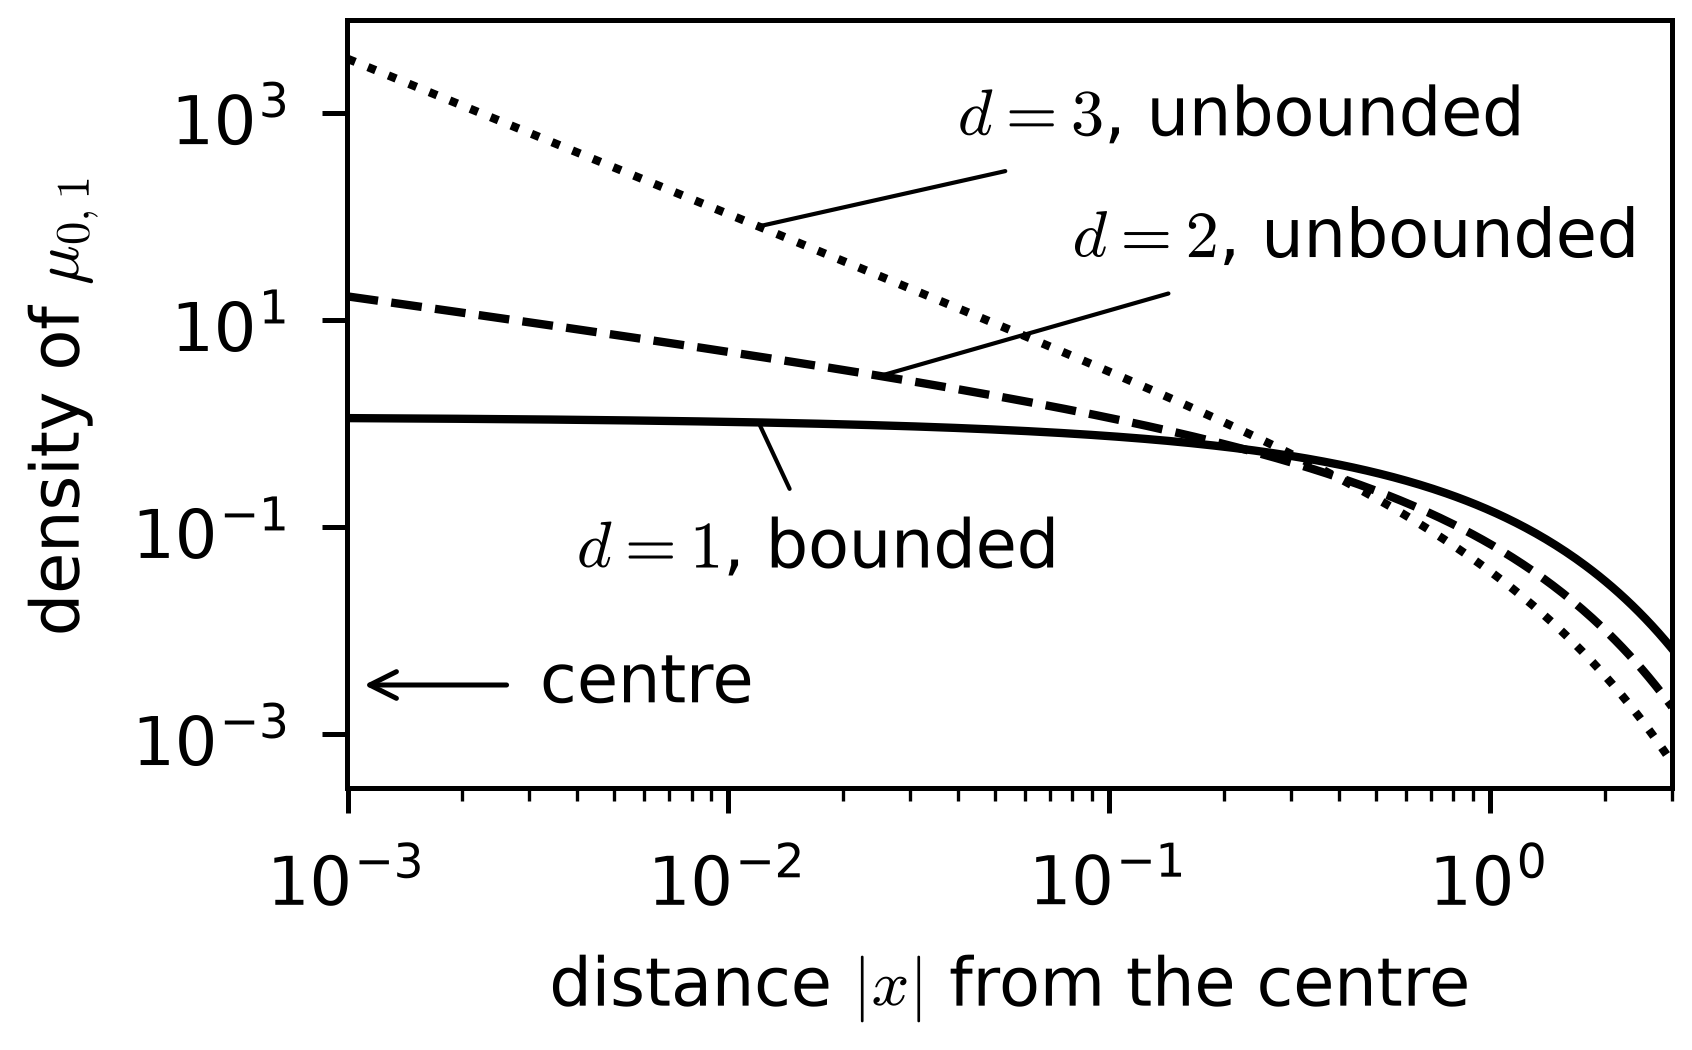
\includegraphics[width=0.45\textwidth]{fig-matern-centre.png}
\caption{The radial density of the \Matern{} kernel $\mu_{0,1}$ of index $\gamma = 3/4$ on
$\RR^d$, $d = 1, 2, 3$, on logarithmic axes, from its closed form \ref{eq:matern-density}. Here
$c = 3/2$. On the line the density is bounded and the curve levels off at the centre. In the
plane and in space it is unbounded, and the curve has the slope $c - d$ there, $-\tfrac12$ in
the plane and $-\tfrac32$ in space. Computed by a script deposited with the paper.}
\label{fig:matern-centre}
\end{figure}

% What the theorem decides comes first, and the comments on its clauses after it (the register
% review, flag 32). A kernel with a Gaussian part: F_d >= a|xi|^2/2, so the transform is
% integrable against every power, and C1 applies with every n.
% Q-0448 (the response to the second external round; records/affine/reviews/
% VERIFY-round2-mathematics.md, items 7 and 11b, and VERIFY-round2-length-and-exposition.md,
% section 4, item 7). The Gaussian part with its argument in full. Which clauses carry the result
% is said before the statement, with the formula of g_t, which clause (4) takes from a lemma of
% the supplement; that c > 0 only excludes the point mass.
The theorem decides boundedness for the kernels with no Gaussian part. A kernel with a Gaussian
part has a bounded smooth density in every dimension: the exponent of a datum $(a,k_d)$ is at
least $\tfrac12 a|\xi|^2$, so for $a > 0$ the transform is at most $e^{-a|\xi|^2/2}$, and C1
applies with every $n$. In clause (4), $g_t$ is the Gaussian density of variance $t$,
\[
  g_t(x) = (2\pi t)^{-d/2}e^{-|x|^2/2t} , \qquad x \in \RR^d ,\ t > 0 ,
\]
which the statement takes from Lemma~\ref{lem:positive-transform-origin} of \suppl. Here $t$ is
not a scale, and $\int g_t\,d\mu$ is the value at the centre of the kernel blurred by $g_t$.
% Q-0448, the blind draft review (flag 26): the comments on the clauses, which stood here
% before the reader had seen the statement, follow it.

% shared with blueprint thm:origin-boundedness-d
\begin{theorem}[the boundedness threshold in dimension $d$ is the dimension]\label{thm:origin-boundedness-d}
Let $d \ge 1$, let $(0, k_d)$ be an isotropic origin datum in dimension $d$ with Gaussian
coefficient $0$, let $\mu$ be its law, put $c := k_d(0{+}) \in [0,\infty]$ and suppose $c > 0$.
\begin{enumerate}
\item \emph{(The profile at the origin is a decay exponent.)} For every finite $\beta < c$ there
is $C_\beta < \infty$ with
\[
  \bigl|\widehat\mu(\xi)\bigr| \le C_\beta\,(1+|\xi|)^{-\beta}, \qquad \xi \in \RR^d .
\]
\item \emph{(Above the threshold: bounded, and a ladder of derivatives.)} Let $N \ge 0$ be an
integer. If $c > d + N$ then $\mu$ has a density of class $C^N$ on the whole of $\RR^d$, all of
whose partial derivatives of orders $0,\dots,N$ tend to $0$ at infinity. In particular $c > d$
makes the density continuous and bounded, and $c = \infty$ makes it $C^\infty$.
\item \emph{(At and below the threshold, on the subordinated slice: unbounded.)} Suppose the
datum is subordinated, with delay datum $(0,k_{\mathrm I})$ of exponent $F_{\mathrm I}$, that $W$
is a random delay whose law, a probability measure on $[0,\infty)$, has Laplace transform
$e^{-F_{\mathrm I}}$, and that $Z$ is standard normal on $\RR^d$, independent of $W$. Then
$c = 2\,k_{\mathrm I}(0{+})$, $W > 0$ almost surely, $\mu$ is the law of $\sqrt{W}Z$, and $\mu$
has the radial density
\begin{equation}\label{eq:mixture-density}
  p(x) = \int_0^\infty (2\pi u)^{-d/2}e^{-|x|^2/2u}\,\Pr(W \in du) .
\end{equation}
This $p$ is nonincreasing in $|x|$, and
\[
  \lim_{x \to 0} p(x) = (2\pi)^{-d}\int_{\RR^d}\widehat\mu(\xi)\,d\xi
   = \frac{(2\pi)^{-d/2}}{\Gamma(d/2)}\int_0^\infty \sigma^{d/2-1}e^{-F_{\mathrm I}(\sigma)}\,d\sigma ,
\]
finite exactly when $c > d$. If $c \le d$, then for every representative $q$ of $\mu$'s
density, every $\delta > 0$ and every $M$ there is an $x$ with $0 < |x| < \delta$ and
$q(x) > M$: no representative is bounded near the origin.
\item \emph{(At and below the threshold, for every datum: unbounded.)} Suppose $c \le d$. Then
$\int_{\RR^d}\widehat\mu(\xi)\,d\xi = \infty$, and there are no $\delta > 0$ and $M < \infty$ with
$\mu(B) \le M|B|$ for every Borel set $B \subseteq \{|x| < \delta\}$. In particular, for every
representative $q$ of a density of $\mu$, every $\delta > 0$ and every $M$ there is an $x$ with
$0 < |x| < \delta$ and $q(x) > M$. Quantitatively, with $g_t$ the heat kernel of
Lemma~\ref{lem:positive-transform-origin}, there is $C > 0$ with
\[
  \int_{\RR^d} g_t\,d\mu \ge C\,t^{-(d-c)/2} \quad (c < d), \qquad
  \int_{\RR^d} g_t\,d\mu \ge C\,\log\frac1t \quad (c = d), \qquad 0 < t \le 1 ,
\]
and for every $\beta$ with $0 < \beta < c$ there is $C'_\beta$ with
$\int g_t\,d\mu \le C'_\beta\,t^{-(d-\beta)/2}$ for all $t > 0$. And
$\log\int g_t\,d\mu / \log(1/t) \to (d-c)/2$ as $t \downarrow 0$.
\item \emph{(The dichotomy.)} The law $\mu$ has a density bounded near the origin, that is, a
density $q$ with $q(x) \le M$ whenever $|x| < \delta$, for some $\delta > 0$ and $M < \infty$,
exactly when $c > d$.
\end{enumerate}
\end{theorem}

% The laws of the theorem: Theorem thm:isotropic-classification with Lemma
% lem:isotropic-realisation and Proposition prop:isotropic-polar-reading(1) (the register
% review, flag 35: the sketch with C4 and C3 is gone). Why the threshold is the dimension: the
% value at the centre as the integral of the transform, the two bounds on the transform, and
% Lemma lem:positive-transform-origin(2), whose attribution to an observation of Feller is in
% Appendix A, where the lemma is stated.
By Theorem~\ref{thm:isotropic-classification} and
Proposition~\ref{prop:isotropic-polar-reading}, the laws of the theorem are the kernels from scale
zero with no Gaussian part, and they are all the rotation-invariant self-decomposable laws on
$\RR^d$ with no Gaussian part other than the point mass. The hypothesis $c > 0$ only
excludes the point mass: $k_d$ is nonincreasing, so $c$ is its supremum. The result is clause
(5), the threshold. Clauses (1) and (2) are its bounded side: the profile at the origin gives
the decay of the transform, and the decay gives the derivatives. Clause (4) is its unbounded
side, for every datum. Clause (3) is for the subordinated data, the Gaussian variance mixtures
whose mixing law is a delay law of \S\ref{sec:line-bridge}: it adds the density as an explicit
mixture, its value at the centre, and $c$ read off the delay profile,
$c = 2k_{\mathrm I}(0{+})$. $N$ continuous derivatives are enough
for the derivative filters of order up to $N$ built from the kernel to be bounded continuous
functions.

The threshold is the dimension for a reason that is seen in the frequency domain. The value at
the centre of a continuous density is $(2\pi)^{-d}\int_{\RR^d}\widehat\mu(\xi)\,d\xi$ when the
transform is integrable. For finite $c$ and large $|\xi|$ the transform lies between a constant
times $|\xi|^{-c}$ and, for every $\beta < c$, a constant times $|\xi|^{-\beta}$
(Lemma~\ref{lem:isotropic-exponent-log}(1) and clause (1)), so it is integrable exactly when
$c > d$. And a law with a nonnegative transform and a density bounded near the origin has an
integrable transform (Lemma~\ref{lem:positive-transform-origin}(2) of \suppl).

The theorem takes $c$ from the \Levy{} measure in dimension $d$. The corollary reads it, and the
Gaussian coefficient, off the exponent.

% shared with blueprint cor:origin-profile-exponent+a6748e79e77b
\begin{corollary}[the exponent determines the Gaussian coefficient and the profile at the origin]\label{cor:origin-profile-exponent}
Let $d \ge 1$, let $(a, k_d)$ be an isotropic origin datum in dimension $d$, let $F_d$ be its
exponent, and put $c := k_d(0{+}) \in [0,\infty]$.
\begin{enumerate}
\item \emph{(The Gaussian coefficient.)} $F_d(\xi)/|\xi|^2 \to \tfrac12 a$ as $|\xi| \to \infty$.
\item \emph{(The profile at the origin.)} As $|\xi| \to \infty$,
\[
  \frac{F_d(\xi) - \tfrac12 a|\xi|^2}{\log|\xi|} \to c ,
\]
where the limit is $+\infty$ when $c = \infty$. In particular, if $a = 0$ and $\mu$ is the datum's
law, then $-\log|\widehat\mu(\xi)|/\log|\xi| \to c$.
\item \emph{(The same numbers in every dimension.)} Let $d' \ge 1$, let $(a', k'_{d'})$ be an
isotropic origin datum in dimension $d'$ with exponent $F'_{d'}$, and suppose that the two exponents
are one function of the radius: there is a function $F$ on $[0,\infty)$ with $F_d(\xi) = F(|\xi|)$
for every $\xi \in \RR^d$ and $F'_{d'}(\xi') = F(|\xi'|)$ for every $\xi' \in \RR^{d'}$. Then
$a' = a$ and $k'_{d'}(0{+}) = k_d(0{+})$.
\end{enumerate}
\end{corollary}

% The consequence for the classes A_d is drawn from three numbered statements, each cited:
% Proposition prop:line-filtration(1) (the nesting), Proposition prop:isotropic-polar-reading (a
% member of A_d has a datum in dimension d) and clause (5) of the theorem.
For a datum with no Gaussian part, clause (2) is the reading of $c$ as the power at which the
transform falls off, and clause (3) removes the dimension. An exponent
$F \in \mathcal{A}_D$ belongs to $\mathcal{A}_d$ for every $d \le D$
(Proposition~\ref{prop:line-filtration}(1)), and in each of these dimensions $F(|\cdot|)$ is the
exponent of a datum (Proposition~\ref{prop:isotropic-polar-reading}). By clause (3) these data
have one Gaussian coefficient and one $c$, and clause (5) of the theorem holds in each of these
dimensions with that $c$. So a kernel that is bounded on the line can have a spike in the plane.

% The number c for the kernels a reader knows (the register review, flag 11; the scope audit,
% row 20: the stable kernels have c = infinity by Corollary cor:origin-profile-exponent applied
% to the exponent of Proposition prop:isotropic-bridge(3), and nothing else is used). Only what
% the statements give: the Gaussian's datum is (a, 0); for F(r) = 2^(-alpha) r^(2 alpha) with
% 2 alpha < 2, F/r^2 -> 0 gives a = 0 and F/log r -> infinity gives c = infinity; the Poisson
% kernel is 2 alpha = 1 (section 2.3); a member of a Cin ray has the folded profile
% b 1_(0,tau), and the unit member has c = 1 (Corollary cor:line-threshold(2)).
For the kernels that a reader knows, the number $c$ is as follows.
\begin{itemize}
\item The Gaussian has a Gaussian part, and no \Levy{} measure. It is outside the theorem, and
it is bounded and smooth.
\item The stable kernels of index $p < 2$ have an exponent that is a multiple of $r^p$
(Proposition~\ref{prop:isotropic-bridge}(3)). So $F(r)/r^2 \to 0$ and
$F(r)/\log r \to \infty$: by clauses (1) and (2) of the corollary they have no Gaussian part and
$c = \infty$, and they are smooth in every dimension, by clause (2) of the theorem. The Poisson
kernel of \S\ref{sec:line-bridge} is the case $p = 1$.
\item The \Matern{} kernel of index $\gamma$ has $c = 2\gamma$ (Example~\ref{ex:matern} below).
\item On the line the member $b\,\Cin(\tau|\omega|)$ of a $\Cin$ ray has the folded profile
$b\,\mathbf 1_{(0,\tau)}$, so $c = b$, and the unit member sits at the threshold
(Corollary~\ref{cor:line-threshold}(2)).
\end{itemize}

An unbounded density could be unbounded at many points. The next proposition says that it is
unbounded at the centre only: the density of every kernel from scale zero, with or without a
Gaussian part, is radially nonincreasing, and so finite at every positive radius.

% shared with blueprint prop:isotropic-radial-monotone+d19bc0659397
\begin{proposition}[the kernels from scale zero have a radially nonincreasing density]\label{prop:isotropic-radial-monotone}
Let $d \ge 1$.
\begin{enumerate}
\item Let $(\mu_{s,t})$ be an isotropic cascade family in dimension $d$ and let $t > 0$. Then
$\mu_{0,t}$ has a density $p$ with $p(x) = q(|x|)$ for $x \ne 0$, where
$q : (0,\infty) \to [0,\infty)$ is nonincreasing.
\item The same holds for the law of every isotropic origin datum $(a,k_d)$ in dimension $d$ that is
not trivial ($a > 0$, or $k_d$ not almost everywhere $0$).
\end{enumerate}
\end{proposition}

% The name a reader needs to use the statement, and no more (the register review, flag 18; the
% citation audit, note on row 39): the anchor is in section 3.5.
% Q-0448, the blind draft review (flag 16): Watanabe's case as the table of the sources has it,
% with its number, and Wolfe's part named apart from it (the proof of the proposition starts
% from C5; READING-watanabe1983isoperimetric.md, sections 1 to 3).
For the law at each time of a symmetric \Levy{} process whose Gaussian covariance is a multiple
of the identity and whose \Levy{} measure has a radially
nonincreasing density the statement is Watanabe's (\sscite{watanabe1983isoperimetric},
Proposition, p.~488; Table~\ref{tab:in-print}). The proof given here derives it from Wolfe's
theorem C5.

% Q-0448 (the response to the second external round; the author's decision of 2026-10-13 that
% nothing is stated twice; records/affine/reviews/VERIFY-round2-length-and-exposition.md,
% section 4, items 8 and 9). The rate is stated once in the main text, through the polar
% profile. The rate through the transform, prop:origin-rate-d, is a lemma of the supplement,
% from which the proof of the rate through the profile starts. The two statements from which
% the rate takes its constants, prop:isotropic-exponent-profile and
% lem:exponent-profile-constant, are stated here, before it, verbatim, with the markers and
% pins they had in Appendix A. The lead defines "varies slowly", "asymptotic" and the constant
% R(d,c) of the Riesz kernel, which the statements below take from that lemma.
The rest of the subsection gives the rate of the spike, computed from the \Levy{} measure. A
positive function $L$ \emph{varies slowly}
at infinity when $L(\lambda\rho)/L(\rho) \to 1$ as $\rho \to \infty$ for every $\lambda > 0$, as
a constant or a logarithm does, and at $0$ when the same holds as its argument decreases to
$0$. Two functions are \emph{asymptotic}, written $f \sim g$, when their quotient tends to $1$.
The density at distance $s$ from the centre is governed by the transform at the frequencies up
to about $1/s$. For the pure power $|\xi|^{-c}$ with $c < d$ this is exact: its inverse Fourier
transform is the Riesz kernel $R(d,c)\,|x|^{c-d}$, with
\[
  R(d,c) := \frac{\Gamma\bigl(\tfrac{d-c}{2}\bigr)}{2^{c}\,\pi^{d/2}\,\Gamma\bigl(\tfrac c2\bigr)} .
\]
The transform of a kernel with a finite $c$ need not be a constant times $|\xi|^{-c}$. The next
proposition says what it is asymptotic to: the power $|\xi|^{-c}$ times a constant and a factor $K(1/|\xi|)$
that varies slowly, both computed from the polar profile. The lemma after it gives in closed
form the one constant that depends on the dimension alone, $\varkappa_d$.

% shared with blueprint prop:isotropic-exponent-profile+f9bd366628e2
\begin{proposition}[the exponent at infinity through the polar profile]\label{prop:isotropic-exponent-profile}
Let $d \ge 1$, let $(0,k_d)$ be an isotropic origin datum in dimension $d$ with Gaussian
coefficient $0$ and $0 < c := k_d(0{+}) < \infty$, let $F_d$ be its exponent, put
$C_k := \int_1^\infty k_d(r)\,dr/r$, and let $e$ be a unit vector of $\RR^d$. Write
$\Cin(X) = \int_0^X (1 - \cos u)\,du/u$ and put
\[
  K(x) := \exp\Bigl[\int_x^1 \bigl(c - k_d(u)\bigr)\,\frac{du}{u}\Bigr] \qquad (0 < x \le 1) .
\]
\begin{enumerate}
\item \emph{(The factor.)} $K$ is continuous and nonincreasing on $(0,1]$, with
$1 = K(1) \le K(x) \le x^{-c}$. For every $a > 0$, $K(ax)/K(x) \to 1$ as $x \downarrow 0$; the
quotient is defined for $0 < x \le \min\{1, 1/a\}$. If $\int_0^1 (c - k_d(u))\,du/u < \infty$,
then $K(x)$ increases, as $x \downarrow 0$, to the finite limit
\[
  K(0{+}) := \exp\int_0^1 \bigl(c - k_d(u)\bigr)\,\frac{du}{u} \;\ge\; 1 .
\]
If the integral diverges, then $K(x) \to \infty$ as $x \downarrow 0$, and $K(0{+}) := \infty$.
\item \emph{(Two constants.)} The limit
\[
  g_\infty := \lim_{X\to\infty}\bigl(\Cin(X) - \log X\bigr)
\]
exists, and $-3 \le g_\infty \le \tfrac{13}{4}$. The function
$\eta \mapsto \log|\langle e,\eta\rangle|$ is integrable on $S^{d-1}$ for $\sigma_{d-1}$, and
\[
  \lambda_d := \frac{1}{|S^{d-1}|}\int_{S^{d-1}}\log|\langle e,\eta\rangle|\,\sigma_{d-1}(d\eta)
  \in (-\infty, 0]
\]
does not depend on $e$, with $\lambda_1 = 0$. Put $\varkappa_d := g_\infty + \lambda_d$.
\item \emph{(The exponent.)} As $\rho \to \infty$,
\[
  F_d(\rho e) - \bigl(c\log\rho - \log K(1/\rho) + C_k\bigr) \to c\,\varkappa_d ,
  \qquad\text{that is}\qquad
  \frac{e^{-F_d(\rho e)}}{e^{-C_k - c\varkappa_d}\,\rho^{-c}\,K(1/\rho)} \to 1 .
\]
Moreover, for every $\rho \ge 1$,
\[
  c\,(\lambda_d - 3) \;\le\; F_d(\rho e) - \bigl(c\log\rho - \log K(1/\rho) + C_k\bigr)
  \;\le\; \tfrac{13}{4}\,c .
\]
More generally, for every $\rho > 0$,
\[
  c\,(\lambda_d - 3) \;\le\; F_d(\rho e) - \int_{1/\rho}^{\infty}k_d(r)\,\frac{dr}{r}
  \;\le\; \tfrac{13}{4}\,c ,
\]
and for $\rho \ge 1$ the integral equals $c\log\rho - \log K(1/\rho) + C_k$.
\item \emph{(When the transform is comparable to a power.)} For every $\xi$ with $|\xi| \ge 1$,
\[
  e^{-13c/4 - C_k}\,K(1/|\xi|) \;\le\; |\xi|^{c}\,e^{-F_d(\xi)} \;\le\;
  e^{c(3-\lambda_d) - C_k}\,K(1/|\xi|) .
\]
So $|\xi|^{c}e^{-F_d(\xi)}$ is bounded on $\{|\xi| \ge 1\}$ if and only if
$\int_0^1 (c - k_d(u))\,du/u < \infty$, and then it tends to
$e^{-C_k - c\varkappa_d}\,K(0{+})$ as $|\xi| \to \infty$.
\end{enumerate}
\end{proposition}

% shared with blueprint lem:exponent-profile-constant+ab60b01e109d
\begin{lemma}[the constant of the exponent in closed form]\label{lem:exponent-profile-constant}
Let $\psi := \Gamma'/\Gamma$ be the digamma function on $(0,\infty)$ and
$\gamma_{\mathrm E} := -\psi(1) = -\Gamma'(1)$ Euler's constant. For an integer $d \ge 1$ let
$g_\infty$, $\lambda_d$ and $\varkappa_d = g_\infty + \lambda_d$ be the constants of
Proposition~\ref{prop:isotropic-exponent-profile}(2).
\begin{enumerate}
\item $g_\infty = \gamma_{\mathrm E}$.
\item $\lambda_d = \tfrac12\bigl[\psi(\tfrac12) - \psi(\tfrac d2)\bigr]$.
\item Hence
\[
  \varkappa_d = \gamma_{\mathrm E} + \tfrac12\bigl[\psi(\tfrac12) - \psi(\tfrac d2)\bigr]
   = \tfrac12\bigl(\gamma_{\mathrm E} - \psi(\tfrac d2)\bigr) - \log 2 ,
\]
so that $\varkappa_1 = \gamma_{\mathrm E}$, $\varkappa_2 = \gamma_{\mathrm E} - \log 2$,
$\varkappa_3 = \gamma_{\mathrm E} - 1$, and $\varkappa_{d+2} = \varkappa_d - 1/d$ for every
$d \ge 1$.
\item \emph{(The constants in closed form.)} For real numbers $c > 0$ and $C$,
\[
  e^{-C - c\varkappa_d}
   = 2^{c}\exp\Bigl(-C - \tfrac c2\bigl(\gamma_{\mathrm E} - \psi(\tfrac d2)\bigr)\Bigr) .
\]
Consequently, with $R(d,c)$ the constant of Lemma~\ref{prop:origin-rate-d}(1) for $0 < c < d$,
\[
  R(d,c)\,e^{-C - c\varkappa_d}
   = \frac{\Gamma\bigl(\tfrac{d-c}{2}\bigr)}{\pi^{d/2}\,\Gamma\bigl(\tfrac c2\bigr)}\,
     \exp\Bigl(-C - \tfrac c2\bigl(\gamma_{\mathrm E} - \psi(\tfrac d2)\bigr)\Bigr),
\]
and
\[
  (2\pi)^{-d}\,|S^{d-1}|\,e^{-C - d\varkappa_d}
   = \frac{2}{\pi^{d/2}\,\Gamma\bigl(\tfrac d2\bigr)}\,
     \exp\Bigl(-C - \tfrac d2\bigl(\gamma_{\mathrm E} - \psi(\tfrac d2)\bigr)\Bigr) .
\]
\end{enumerate}
\end{lemma}

The proposition has no hypothesis on $c$ against $d$, so it describes the transform above the
threshold as well. Of $g_\infty$ it uses only that the limit exists, with the bounds of clause
(2), and the lemma gives its value. When $c \le d$ the density follows the transform as the
Riesz kernel follows the pure power. For $c < d$ the density $q(s)$ at distance $s$ from the
centre is asymptotic, as $s \downarrow 0$, to $R(d,c)\,s^{-d}\,\widehat\mu(e/s)$, with $e$ a
unit vector. This step from the transform to the density is a Tauberian theorem,
Lemma~\ref{prop:origin-rate-d}(1) of \suppl, from which the statements here cite the constant
$R(d,c)$, and \S\ref{sec:isotropic-sources} says where it is in print. At $c = d$ the transform is at the edge of integrability, and an integral of $K$
takes the place of the power. In the statement $s$ is a distance from the centre, not a scale.
% Q-0448, the blind draft review of the split (flags 3 and 27): the paragraph states clause (1)
% of Lemma prop:origin-rate-d for the density, which the paper's reader does not have, and no
% longer clause (1) of the proposition below with a second definition of A.

% shared with blueprint prop:origin-rate-profile-d+2165aacf61aa
\begin{proposition}[the rate at the centre through the polar profile]\label{prop:origin-rate-profile-d}
Let $d \ge 1$, let $(0, k_d)$ be an isotropic origin datum in dimension $d$ with Gaussian
coefficient $0$, let $\mu$ be its law, and suppose that $c := k_d(0{+})$ satisfies $0 < c \le d$.
Let $C_k$, $K$ and $\varkappa_d$ be as in Proposition~\ref{prop:isotropic-exponent-profile}, let $|S^{d-1}|$
be the surface measure of the unit sphere and $V_d$ the volume of the unit ball, and put
\[
  A := e^{-C_k - c\,\varkappa_d} .
\]
The law $\mu$ has a density $p$ with $p(x) = q(|x|)$ for $x \ne 0$, where
$q : (0,\infty) \to [0,\infty)$ is nonincreasing. Let $q$ be any such function. All limits are as
$s \downarrow 0$.
\begin{enumerate}
\item \emph{(Below the threshold.)} Let $c < d$, let $R(d,c)$ be the constant of
Lemma~\ref{prop:origin-rate-d}(1), and put $Q := R(d,c)\,A$. Then
\[
  \frac{q(s)}{Q\,s^{c-d}\,K(s)} \to 1
  \qquad\text{and}\qquad
  \frac{\mu(\{|x| \le s\})}{Q\,|S^{d-1}|\,c^{-1}\,s^{c}\,K(s)} \to 1 .
\]
\item \emph{(When a pure power holds.)} Let $c < d$. If
$\int_0^1 (c - k_d(u))\,du/u < \infty$, then $q(s)\,s^{d-c} \to Q\,K(0{+})$, a finite positive
number, and there is $C < \infty$ with $q(s) \le C\,s^{c-d}$ for every $s > 0$. If the integral
diverges, then $q(s)\,s^{d-c} \to \infty$, and there is no such $C$.
\item \emph{(At the threshold.)} Let $c = d$, and put
\[
  \mathcal{L}(s) := \int_s^1 K(y)\,\frac{dy}{y} \quad (0 < s \le 1), \qquad
  B := (2\pi)^{-d}\,|S^{d-1}|\,A .
\]
Then
\[
  \frac{q(s)}{B\,\mathcal{L}(s)} \to 1
  \qquad\text{and}\qquad
  \frac{\mu(\{|x| \le s\})}{B\,V_d\,s^{d}\,\mathcal{L}(s)} \to 1 .
\]
Moreover $\log(1/s) \le \mathcal{L}(s) \le K(s)\log(1/s)$ for $0 < s \le 1$. If
$\int_0^1 (d - k_d(u))\,du/u < \infty$, then
\[
  \frac{\mathcal{L}(s)}{\log(1/s)} \to K(0{+})
  \qquad\text{and}\qquad
  \frac{q(s)}{\log(1/s)} \to B\,K(0{+}) ,
\]
both limits finite and positive. If the integral diverges, then
$\mathcal{L}(s)/\log(1/s) \to \infty$ and $q(s)/\log(1/s) \to \infty$.
\end{enumerate}
\end{proposition}

% After the statement: the closed forms of Q and B are the second and third displays of clause
% (4) of Lemma lem:exponent-profile-constant at C = C_k. The peak of the record of a point
% source is read once from the limits for the mass of a ball: mu({|x| <= s}) over V_d s^d, with
% |S^{d-1}| = d V_d ("the peak of the opening" until Q-0448; the second external round, review
% C, R2). The profile with an unbounded factor is the blind referee's, with K in closed form
% (records/affine/check-q0428-prose-values.py, part (b)). The dependence on the scale is a
% computation of the prose, listed as such in the supplement (the same script, part (g)).
% Q-0448, the blind draft review (flag 27): the closed forms of Q and B are the second and the
% third display of clause (4) of the lemma, at C = C_k (with c = d in the third), and are not
% displayed again.
Lemma~\ref{lem:exponent-profile-constant}(4) at $C = C_k$ gives $Q$ and $B$ in closed form.
So the kernel at its centre is computed from its \Levy{} measure: the power is $c - d$, the
factor $K(s)$ is one integral of the polar profile over $(s,1)$, and the constant depends on
$c$, on $d$ and on the profile beyond radius $1$. By clauses (2) and (3) the density is
asymptotic to a constant times $|x|^{c-d}$, or times $\log(1/|x|)$ at the threshold, exactly
when $K$ is bounded. The
limits for the mass of a ball give the peak of the record of a point source, the mass of the
recording cell divided by its volume. For a cell of radius $s$ round the centre it is
asymptotic to $(d/c)\,Q\,s^{c-d}K(s)$ for $c < d$ and to $B\,\mathcal{L}(s)$ for $c = d$,
because $|S^{d-1}| = d\,V_d$.

% Q-0448 (VERIFY-round2-length-and-exposition.md, section 4, item 9; the author's decision that
% nothing is stated twice): the example in one place, after the rate, where it had four (after
% the corollary, after each form of the rate, and in section 3.4). It names its delay law, so
% that the hypotheses of the clauses it uses are seen to be met. The closed form is Fischer et
% al., the display after (24), p. 241, at mu = theta = 0, s = gamma and Sigma = I
% (READING-fischer2025variance.md), and it is the mixture eq:mixture-density against the gamma
% law (records/affine/check-matern-rate-constants.py, part (a)). It is the Bessel kernel
% G_{2 gamma} of Aronszajn and Smith at range 1/sqrt 2, p(x) = 2^{d/2} G_{2 gamma}(sqrt 2 x), for
% every gamma > 0 ((4,1), p. 416; READING-aronszajn1961theory.md, section 3), and the two
% regimes at the centre are their (4,2), rescaled. The coefficient of the spike is read from
% the identity A K(0+) = 2^gamma, which holds because the transform is asymptotic both to
% A rho^(-c) K(1/rho) (Proposition prop:isotropic-exponent-profile(3)) and to
% 2^gamma rho^(-2 gamma); the rate through the transform is not needed. The numbers of the
% table: records/affine/check-q0448-matern-table.py, with its output beside it.
\begin{example}[the \Matern{} kernels]\label{ex:matern}
The \Matern{} kernel of index $\gamma > 0$ is the kernel from scale zero with exponent
$F(r) = \gamma\log(1 + r^2/2)$ (Proposition~\ref{prop:isotropic-bridge}(2)). Here
$F(r) = F_{\mathrm I}(r^2/2)$ with $F_{\mathrm I}(\sigma) = \gamma\log(1+\sigma)$, which is
causally admissible with delay profile $k_{\mathrm I}(u) = \gamma e^{-u}$, and its delay law is
the gamma law of shape $\gamma$, with density $u^{\gamma-1}e^{-u}/\Gamma(\gamma)$. So $F$ lies in
every $\mathcal{A}_d$ (Proposition~\ref{prop:line-filtration}(2)), its datum in each dimension
is subordinated (Lemma~\ref{lem:delay-polar-profile}), and clause (3) of
Theorem~\ref{thm:origin-boundedness-d} applies with a gamma-distributed $W$. It gives
$c = 2k_{\mathrm I}(0{+}) = 2\gamma$. So the kernel is bounded exactly when $\gamma > d/2$: for
$\gamma > \tfrac12$ on the line, for $\gamma > 1$ in the plane and for $\gamma > \tfrac32$ in
space. The mixture \ref{eq:mixture-density} is here, at scale $1$
(\sscite{fischer2025variance}, (24) and the display after it, p.~241),
\begin{equation}\label{eq:matern-density}
  p(x) = \frac{2}{(2\pi)^{d/2}\,\Gamma(\gamma)}
    \Bigl(\frac{|x|}{\sqrt2}\Bigr)^{\gamma - d/2} K_{\gamma - d/2}\bigl(\sqrt2\,|x|\bigr) ,
\end{equation}
with $K_\nu$ the modified Bessel function of the second kind. For $\gamma > d/2$ this is the
\Matern{} function of smoothness $\gamma - d/2$ and range $1/\sqrt2$ (\sscite{porcu2024matern},
(9) of the arXiv version), so the kernel is bounded exactly where it is a \Matern{} covariance
function. For every $\gamma > 0$ it is the Bessel kernel of potential theory, dilated by
$1/\sqrt2$ (\sscite{aronszajn1961theory}, (4,1), p.~416). The authors of the Bessel scale
space (\S\ref{sec:introduction}) note that the
kernel with $2\gamma = d + 1$ is continuous and not differentiable at the centre, and the kernel
with $2\gamma = d + 3$ twice continuously differentiable (\sscite{burgeth2005bessel}, p.~87).
The continuity and the two derivatives are the cases $N = 0$ and $N = 2$
of clause (2) of Theorem~\ref{thm:origin-boundedness-d}.
% Q-0448, the blind draft review (flags 12 and 37): which kernel of the Bessel scale space this
% is, is said once, in section 1; "not differentiable" is not a case of clause (2), which
% gives derivatives and is silent on the next one.

By \ref{eq:polar-profile-d} with the delay profile $\gamma e^{-u}$, the polar profile of the
kernel is
\[
  k_d(r) = \frac{4\gamma}{\Gamma(d/2)}\Bigl(\frac{r}{\sqrt2}\Bigr)^{d/2}K_{d/2}\bigl(\sqrt2\,r\bigr) ,
\]
which is $2\gamma e^{-\sqrt2\,r}$ on the line and $2\gamma(1 + \sqrt2\,r)e^{-\sqrt2\,r}$ in
space. For it the integral $\int_0^1 (c - k_d(u))\,du/u$ is finite, so the factor $K$ is
bounded, and for $\gamma < d/2$ the spike is a pure power
(Proposition~\ref{prop:origin-rate-profile-d}(2)). Its coefficient needs no integral. The
transform $(1 + \rho^2/2)^{-\gamma}$ is asymptotic to $2^{\gamma}\rho^{-2\gamma}$, and to
$A\,\rho^{-c}K(1/\rho)$ by Proposition~\ref{prop:isotropic-exponent-profile}(3), so
$A\,K(0{+}) = 2^{\gamma}$ in every dimension. Hence, as $x \to 0$,
\[
  p(x) \sim \frac{\Gamma(d/2 - \gamma)}{2^{\gamma}\pi^{d/2}\,\Gamma(\gamma)}\,|x|^{2\gamma - d}
  \quad \bigl(\gamma < \tfrac d2\bigr), \qquad
  p(x) \sim \frac{2}{(2\pi)^{d/2}\,\Gamma(d/2)}\,\log\frac{1}{|x|}
  \quad \bigl(\gamma = \tfrac d2\bigr) ,
\]
the coefficients being $Q\,K(0{+})$ and $B\,K(0{+})$. The second case is index $1$ in the
plane. Both are the behaviour of the closed form \ref{eq:matern-density} at the centre
(\sscite{aronszajn1961theory}, (4,2), p.~416, in the present scaling). Table~\ref{tab:matern}
has the numbers for $\gamma = 3/4$, the kernel of Figure~\ref{fig:matern-centre}.
\end{example}

\begin{table}[!htb]
\centering
\small
\begin{tabular}{@{}ccccccl@{}}
\toprule
$d$ & $c - d$ & $C_k$ & $K(0{+})$ & $A$ & $Q$ & the density at the centre \\
\midrule
$1$ & $\tfrac12$ & $0.171$ & $4.741$ & $0.355$ & & bounded, with $p(0) \approx 1.180$ \\
$2$ & $-\tfrac12$ & $0.359$ & $2.023$ & $0.831$ & $0.277$ & $p(x) \sim 0.560\,|x|^{-1/2}$ \\
$3$ & $-\tfrac32$ & $0.535$ & $1.524$ & $1.104$ & $0.0701$ & $p(x) \sim 0.107\,|x|^{-3/2}$ \\
\bottomrule
\end{tabular}
\caption{The \Matern{} kernel $\mu_{0,1}$ of index $\gamma = 3/4$, at scale $1$ in the gauge
$\chi(t) = t$, for which $c = 3/2$, in dimensions $1$,
$2$ and $3$: the constants of Propositions~\ref{prop:isotropic-exponent-profile}
and~\ref{prop:origin-rate-profile-d}, and the density at the centre. In each dimension
$A\,K(0{+}) = 2^{3/4}$. Computed by a script deposited with the paper.}
\label{tab:matern}
\end{table}

The factor need not be bounded. Let $0 < c < d$, and let $k_d(u) = c\,(1 - 1/(2 + \log(1/u)))$
for $0 < u \le 1$, continued beyond radius $1$ by a nonincreasing function with $C_k < \infty$.
The profile approaches $c$ like $1/\log(1/u)$, the integral diverges, and
$K(x) = (1 + \tfrac12\log(1/x))^{c}$. So $q(s) \sim Q\,s^{c-d}\,(1 + \tfrac12\log(1/s))^{c}$:
the spike exceeds every multiple of the pure power, by a power of a logarithm.

The statements are for one law, and a family has a kernel for each scale. The kernel from scale
zero to scale $t$ is the dilation of the law by $\chi(t)$, with density
$\chi(t)^{-d}\,p(x/\chi(t))$. For $c < d$ this is asymptotic at the centre to
$\chi(t)^{-c}\,Q\,|x|^{c-d}K(|x|)$, because $K$ varies slowly. So the power and the factor are
the same at every scale, and the constant is multiplied by $\chi(t)^{-c}$. The radius $1$ in $K$
and in $C_k$ is the unit of length at the scale where $\chi(t) = 1$.

% The two bounds are stated in Appendix A (Propositions prop:origin-lower-bound-d and
% prop:origin-upper-bound-d). The paragraph says what each gives that the rate does not, with
% its hypotheses, why the lower bound needs d >= 2 and what holds on the line, what the
% constants depend on, and that together they give the order (the register review, flag 30).
% The last two sentences keep c < d and c = d apart (the scope audit, row 3: at c = d a bound at
% the power c would be a bounded density, which Theorem thm:origin-boundedness-d(4) excludes).
% Q-0448, the blind draft review, the length: the paragraph keeps what each bound gives. What
% the appendix says after each statement (why the lower bound needs d >= 2, and the line) and
% what the comment on clause (2) of the rate says (when a bound at the power c itself holds)
% are not repeated here.
Two bounds complement the rate, and \S\ref{app:further-statements} states them. An
asymptotic equivalence gives no radius on which an inequality holds and no constant for it. For
$d \ge 2$ and a finite $c$ the kernel is bounded from below near its centre:
$\mu(E) \ge c_1\int_E |x|^{c-d}\,dx$ for every Borel set $E$ in a ball $\{|x| < \delta\}$, with
$\delta$ and $c_1$ given in terms of $d$, of $c$ and of the polar profile
(Proposition~\ref{prop:origin-lower-bound-d}). For $c \le d$ and every $\beta < c$ the
density is bounded from above at every radius: $q(s) \le (A_\beta/V_d)\,s^{\beta-d}$, with $V_d$
the volume of the unit ball and a constant $A_\beta$ that \suppl{} gives in closed form
(Proposition~\ref{prop:origin-upper-bound-d}; \S\ref{supp:proofs-origin}). For $d \ge 2$ and $c \le d$ the
two bounds together give the
order of the density at the centre, $\log p(x)/\log(1/|x|) \to d - c$ (its clause (3)).

% Q-0448, the blind draft review (flags 5 and 6): the lead says what a stage does to a record,
% in the two cases of the proposition; what was said "in plain words" after the statement is
% here, and the comment after the statement keeps what the lead does not say. The Matern case
% gamma = 1, which stood in Example ex:matern before the proposition was stated, follows it.
\paragraph{The stages.} The statements above are about the kernels from scale zero. A stage
$\mu_{s,t}$ with $s > 0$, which is what a cascade applies to a record, is a residual of such a
kernel (\S\ref{sec:line-axioms}), and need not be a dilation of it. When the kernels have no Gaussian
part and $c$ is finite, a stage does not blur everything. It returns the fraction
$(\chi(s)/\chi(t))^c$ of the record at scale $s$ unchanged, and adds a blur of that record by a
density of mass $1 - (\chi(s)/\chi(t))^c$. With a Gaussian part, or with $c = \infty$, as for
the stable kernels, a stage is a blur by a density.

% Q-0448 (review D, R1, of the second external round; records/affine/NODES-q0434.md, section 2;
% the author's decision of 2026-10-13 that the stages are machine-checked, by queue item
% Q-0447). One proposition for the three blueprint nodes of Q-0434 on the stages:
%   clause (1)  lem:isotropic-stage-levy-measure, for l = chi(s) and L = chi(t): its clause (1)
%               and its last sentence (the transform of the stage, the mass), which is the form
%               the node itself gives for a family; the node's statement for a datum and two
%               numbers 0 < l < L is the first paragraph of the proof;
%   clause (2)  prop:isotropic-stage-atom, its four clauses as the items (a) to (d);
%   clause (3)  prop:isotropic-stage-density, its three clauses as the items (a) to (c), and
%               its closing sentence, which closes the proposition.
% Nothing is added to the three statements and nothing of the second and third is left out.
% Pinned against the three nodes, statement and proof, after reading.
% Machine-checked since the Lean of Q-0447 was merged (the joining step of Q-0448): the three
% nodes are \leanok, the proposition is under the first list of section 1.1, its proof is in the
% supplement (supp-proofs.tex inputs proof-stages.tex), and it has an item in the list of
% section S4 and a row in the table of Appendix B (records/affine/gen-verification-table.py,
% ROWS; axioms-iso-all-declarations.py, TABLE1). The proofs of record's closing paragraphs,
% which Q-0447 rewrote, are not printed, as for every proof; the one sentence of them that is
% (after item (d) of clause (2)) follows the blueprint, and the marker is pinned again.
% shared with blueprint lem:isotropic-stage-levy-measure@db25bbbf95b6+26ef2b33d950, prop:isotropic-stage-atom@e901f7de9352+6df4676673ea, prop:isotropic-stage-density@83e3e3ecc9fb+ae42a1d0f900
\begin{proposition}[the stages of a cascade]\label{prop:isotropic-stages}
Let $d \ge 1$, let $(\mu_{s,t})_{0 \le s \le t}$ be an isotropic cascade family in dimension $d$,
and let $\chi$ be a gauge and $F \in \mathcal{A}_d$ with $F \not\equiv 0$ that satisfy
\ref{eq:isotropic-classification} (Theorem~\ref{thm:isotropic-classification}). Let $(a, k_d)$ be
an isotropic origin datum in dimension $d$ with exponent $\xi \mapsto F(|\xi|)$, put
$c := k_d(0{+}) \in [0,\infty]$, let $0 < s < t$, and put
$\lambda := \chi(s)/\chi(t) \in (0,1)$. The \emph{\Levy{} measure of the stage} is the measure
$\nu_{s,t}$ on $\RR^d \setminus \{0\}$ with the density
$\kappa_{s,t}(|x|)\,\bigl(|S^{d-1}|\,|x|^d\bigr)^{-1}$, where
\[
  \kappa_{s,t}(r) := k_d\Bigl(\frac{r}{\chi(t)}\Bigr) - k_d\Bigl(\frac{r}{\chi(s)}\Bigr)
  \qquad (r > 0) .
\]
\begin{enumerate}
\item \emph{(The \Levy{} measure of a stage.)} $\kappa_{s,t} \ge 0$, the measure $\nu_{s,t}$ is
rotation invariant, and $\int_{\RR^d}(|x|^2 \wedge 1)\,\nu_{s,t}(dx) < \infty$. The transform of
the stage is
\begin{equation}\label{eq:stage-transform}
  \widehat\mu_{s,t}(\xi) = \exp\Bigl[-\tfrac12 a\bigl(\chi(t)^2 - \chi(s)^2\bigr)|\xi|^2
     - \int_{\RR^d}\bigl(1 - \cos\langle\xi,x\rangle\bigr)\,\nu_{s,t}(dx)\Bigr],
  \qquad \xi \in \RR^d ,
\end{equation}
and $\nu_{s,t}(\RR^d \setminus \{0\}) = c\,\log\bigl(\chi(t)/\chi(s)\bigr)$, in $[0,\infty]$. So
$\nu_{s,t}$ is a finite measure exactly when $c < \infty$.
\item \emph{(No Gaussian part and a finite $c$: a point mass at the centre.)} Suppose that
$a = 0$ and that $c$ is finite, and put $m := c\,\log(\chi(t)/\chi(s))$. Then $c > 0$, and:
\begin{enumerate}
\item[(a)] \emph{(The stage is compound Poisson.)}
$\mu_{s,t} = e^{-m}\sum_{n \ge 0}\nu_{s,t}^{*n}/n!$, with $\nu_{s,t}^{*0} = \delta_0$, and
$e^{-m} = \lambda^c$.
\item[(b)] \emph{(A point mass at the centre and a smoothing part.)} The measure
$\eta_{s,t} := \lambda^c\sum_{n \ge 1}\nu_{s,t}^{*n}/n!$ is absolutely continuous with respect
to Lebesgue measure, of total mass $1 - \lambda^c$, and
\[
  \mu_{s,t} = \lambda^c\,\delta_0 + \eta_{s,t} .
\]
So $\mu_{s,t}(\{0\}) = (\chi(s)/\chi(t))^c \in (0,1)$, and $\mu_{s,t}$ has no density.
\item[(c)] \emph{(The operator.)} With $p_{s,t} \ge 0$ a density of $\eta_{s,t}$, an integrable
function of integral $1 - \lambda^c$, the operator of the stage is
\[
  \mu_{s,t} * f = \Bigl(\frac{\chi(s)}{\chi(t)}\Bigr)^{c} f + p_{s,t} * f ,
  \qquad f \in L^1(\RR^d) .
\]
\item[(d)] \emph{(Not self-decomposable.)} $\mu_{s,t}$ is not self-decomposable.
\end{enumerate}
\item \emph{(Infinitely divisible; the stages with a density.)}
\begin{enumerate}
\item[(a)] $\mu_{s,t}$ is infinitely divisible and has the generating triplet
$\bigl(a(\chi(t)^2 - \chi(s)^2)\,I,\ \nu_{s,t},\ 0\bigr)$: its Gaussian part has the variance
$a(\chi(t)^2 - \chi(s)^2)$ in every direction, and its \Levy{} measure has the polar profile
$\kappa_{s,t}$ and the mass $c\,\log(\chi(t)/\chi(s))$.
\item[(b)] If $a = 0$ and $c = \infty$, then $\mu_{s,t}$ is absolutely continuous with respect
to Lebesgue measure. In particular it has no point mass.
\item[(c)] If $a > 0$, then $\mu_{s,t}$ has a bounded density of class $C^\infty$, all of whose
partial derivatives are bounded.
\end{enumerate}
\end{enumerate}
So a stage $\mu_{s,t}$ with $0 < s < t$ has a point mass at the centre exactly when the datum
has no Gaussian part and a finite profile at the origin, and it has a density in the two other
cases.
\end{proposition}

Clauses (1) and (3) give the stage as a law: it is infinitely divisible, and its \Levy{}
measure is the difference of two dilations of that of the kernel. The fraction of clause (2) tends to $0$
as $s \downarrow 0$, and the kernels from scale zero have no point mass. The number $c$, the
ratio $\chi(t)/\chi(s)$ and the product $a\,\chi(t)^2$ are the same for every pair
$(\chi, F)$ of the family, by the uniqueness clause of
Theorem~\ref{thm:isotropic-classification}. For the \Matern{} kernels of
Example~\ref{ex:matern}, in the gauge $\chi(t) = t$ of
Proposition~\ref{prop:isotropic-bridge}, the fraction is $(s/t)^{2\gamma}$. At $\gamma = 1$ the
stage is $\mu_{s,t} = (s/t)^2\delta_0 + (1 - (s/t)^2)\,\mu_{0,t}$ in every dimension, a point
mass and a multiple of the kernel at scale $t$: its transform is
$(1 + s^2\sigma)/(1 + t^2\sigma) = (s/t)^2 + (1 - (s/t)^2)/(1 + t^2\sigma)$ at
$\sigma = |\xi|^2/2$.

\subsection{The dimension filtration}\label{sec:isotropic-filtration}

% Q-0428, the fixes round (records/affine/REPOSITIONING-paper-iso-round2-fixes.md; the register
% review of sections 3.3 to 4, structural change 3). The subsection states what it quotes, once.
% Three statements: the dictionary (prop:radial-dictionary, with what it is in words before it and
% the Matern exponent put through it after it); the test on the Levy measure
% (prop:profile-one-dimension-down, the node that Q-0429 split from the corollary: statements on
% data, no law and no characteristic function), with its two readings in the dictionary
% (cor:dictionary-filtration, the label kept, the statement now those readings only); and the
% separating family (def:filtration-thresholds, then thm:separating-family-critical-values, the
% node of Q-0429 that carries "F^(w) in A_D iff w <= w_D", the strict decrease and the limit).
% thm:filtration-strict and thm:no-cin-ray-in-the-plane are not printed since Q-0448 (section S4
% of the supplement lists their declarations): they are the same facts as the new theorem on
% another footing and as clause (3) of the new proposition. One word per sense: "dimension" for a place in the chain, "step" for the
% profile b 1_(0,tau), "bump" for the box on [1,2] of the separating family.
% Attribution is in section 3.5 (sources.tex), once.
In every dimension an isotropic family is given by the same kind of object, a gauge and an
exponent $F$, a function of one variable: the transform of its kernel from scale zero is
$e^{-F(\chi(t)|\xi|)}$ (Theorem~\ref{thm:isotropic-classification}). The familiar families use one
exponent in every dimension. The Gaussian has $F(r) = \tfrac12 r^2$, and the $\alpha$-scale
spaces, which are written on $\RR^d$ \sscite{duits2004axioms}, have a multiple of
$r^{2\alpha}$ (Proposition~\ref{prop:isotropic-bridge}(3)). This subsection asks whether that is
general. Does the exponent of a family in dimension $d$ give a family in dimension $d + 1$ when
it is read as a function of $|\xi|$? By Theorem~\ref{thm:isotropic-classification} and
Lemma~\ref{lem:isotropic-realisation}, the exponents of the isotropic families in dimension $d$
are exactly the members $F \not\equiv 0$ of the class $\mathcal{A}_d$ of
Proposition~\ref{prop:line-filtration}. The way down is always open, since
$\mathcal{A}_{d+1} \subseteq \mathcal{A}_d$. The way up is not: in every dimension some exponents
are lost. The exponents admitted in every dimension are exactly those of the subordinated
families of \S\ref{sec:line-bridge} (Proposition~\ref{prop:line-filtration}(3)), the \Matern{}
and the stable kernels among them (Proposition~\ref{prop:isotropic-bridge}).

The subsection has three parts. The first matches the exponents of the kernels with no
Gaussian part and a finite $c$ with probability laws on $\RR^d$, and says which of them are
admitted one dimension up. The second is a test on the \Levy{} measure, for every exponent,
with what becomes of the simplest exponent that fails it. The third follows one family of
exponents through the dimensions.

% What the dictionary is, in words, before the statement (the register review, flag 4), and what
% each condition on the law does in terms of the polar profile (flag 28). k_d/c is nonincreasing,
% tends to 1 at radius zero and to 0 at infinity (the second integrability condition of
% Definition def:isotropic-origin-datum); the statement has Pr(|X| > r) = k_d(r+)/c. E log^+ R
% = int_1^infty Pr(R > r) dr/r, by Tonelli. An atom of mass p at the origin changes (c, the law)
% to (c(1 - p), the law conditioned off the origin) and leaves F unchanged (the node's
% annotation, point (iv) of the comment before it). Omega_2 = J_0 and Omega_3(t) = sin t / t:
% records/affine/check-q0428-prose-values.py, part (d).
The first statement is for the kernels of \S\ref{sec:isotropic-origin} with no Gaussian part
and a finite $c$. Their exponents are the members of $\mathcal{A}_d$ that grow like a logarithm,
$F(r)/\log r \to c$ with $0 < c < \infty$ (Corollary~\ref{cor:origin-profile-exponent}). The
\Matern{} kernels are among them, and the Gaussian and the stable kernels are not. Let $k_d$ be
the polar profile of such a kernel. The function $k_d/c$ decreases from $1$ at radius zero to
$0$ at infinity, so it is, up to its values at its jumps, the tail $r \mapsto \Pr(R > r)$ of a
random radius $R > 0$. Let $X$ be that radius in a direction drawn uniformly from the sphere.
The transform of the law of $X$ is a function $\phi(|\xi|)$ of the radius alone, a
\emph{radial characteristic function} on $\RR^d$. Read as a function of a displacement, it is
equally an isotropic correlation function that is valid in $\RR^d$. The proposition says that
$F$ and the pair $(c, \phi)$ determine each other, and that $F$ is admitted one dimension up
exactly when the same function of the radius is still the transform of a probability law on
$\RR^{d+1}$.

In the statement $\Omega_d(t)$ is the mean of $\cos(t\langle e,\eta\rangle)$ over the unit
sphere, the transform along a ray of the uniform law on the sphere: $\Omega_1 = \cos$,
$\Omega_2 = J_0$, the Bessel function of order zero, and $\Omega_3(t) = \sin t/t$. A random
vector $X$ stands for its law, and $\log^+ := \max\{\log, 0\}$. Two conditions are put on the
law. The first, $\mathbb{E}\log^+|X| < \infty$, a \emph{finite logarithmic moment}, is the
condition $\int_1^\infty k_d(r)\,dr/r < \infty$ of Definition~\ref{def:isotropic-origin-datum},
because $\mathbb{E}\log^+|X| = \int_1^\infty \Pr(|X| > r)\,dr/r$. The second, no atom at the
origin, makes $k_d(0{+}) = c$: an atom of mass $p$ there would give the same $F$ with
$c(1-p)$ in place of $c$, so the condition is what makes the pair unique.

% shared with blueprint prop:radial-dictionary+675deea1f81e
\begin{proposition}[the dictionary between $\mathcal{A}_d$ and the radial characteristic functions]\label{prop:radial-dictionary}
Let $d \ge 1$. For $t \ge 0$ put
\[
  \Omega_d(t) := \frac{1}{|S^{d-1}|}\int_{S^{d-1}}\cos\bigl(t\langle e,\eta\rangle\bigr)\,
     \sigma_{d-1}(d\eta) ,
\]
which does not depend on the unit vector $e$; $\Omega_1 = \cos$. Call a random vector $X$ in
$\RR^d$ \emph{rotation invariant} when $QX$ has the law of $X$ for every $Q \in \Orth(d)$. Its
characteristic function is then real and radial,
\[
  \mathbb{E}\,e^{i\langle\xi,X\rangle} = \phi(|\xi|), \qquad
  \phi(r) := \mathbb{E}\,\Omega_d\bigl(r|X|\bigr) \quad (r \ge 0) ,
\]
the function $\phi$ determines the law of $X$, and $X$ has the law of $R\,U$, where $R$ has the
law of $|X|$ and $U$ is uniformly distributed on $S^{d-1}$ and independent of $R$.
\begin{enumerate}
\item \emph{(From a law to an exponent.)} Let $X$ be a rotation-invariant random vector in
$\RR^d$ with $\Pr(X = 0) = 0$, let $\phi$ be as above, and let $0 < c < \infty$. Then
$\int_0^1 (1 - \phi(u))\,du/u < \infty$ if and only if $\mathbb{E}\log^+|X| < \infty$. In that
case the function
\[
  F(r) := c\int_0^r \bigl(1 - \phi(u)\bigr)\,\frac{du}{u} \qquad (r \ge 0)
\]
belongs to $\mathcal{A}_d$: $\xi \mapsto F(|\xi|)$ is the exponent of the isotropic origin datum
$(0,k_d)$ in dimension $d$ with $k_d(r) = c\,\Pr(|X| > r)$. Its profile at the origin is
$k_d(0{+}) = c$, and $F(r)/\log r \to c$ as $r \to \infty$.
\item \emph{(From an exponent to a law.)} Conversely, let $F \in \mathcal{A}_d$ and suppose that
$F(r)/\log r$ has a limit $c \in (0,\infty)$ as $r \to \infty$. Then $F$ is the function of
clause (1) for this $c$ and for a rotation-invariant $X$ with $\Pr(X = 0) = 0$ and
$\mathbb{E}\log^+|X| < \infty$, whose law is unique. Moreover $F$ is continuously differentiable
on $(0,\infty)$, with
\[
  \phi(r) = 1 - \frac{r\,F'(r)}{c} \quad (r > 0), \qquad
  \Pr(|X| > r) = \frac{k_d(r{+})}{c} \quad (r > 0)
\]
for every isotropic origin datum $(0,k_d)$ in dimension $d$ with exponent $\xi \mapsto F(|\xi|)$.
So $(c, \text{the law of } X) \mapsto F$ is a bijection from the pairs of clause (1) with
$\mathbb{E}\log^+|X| < \infty$ onto the set of the $F \in \mathcal{A}_d$ for which $F(r)/\log r$
has a limit in $(0,\infty)$. These are the members of $\mathcal{A}_d$ with Gaussian coefficient
$0$ and profile at the origin in $(0,\infty)$.
\item \emph{(The next dimension.)} Let $F$, $c$, $X$ and $\phi$ be as in clause (1), with
$\mathbb{E}\log^+|X| < \infty$. Then $F \in \mathcal{A}_{d+1}$ if and only if
$\zeta \mapsto \phi(|\zeta|)$, $\zeta \in \RR^{d+1}$, is the characteristic function of a random
vector $X'$ in $\RR^{d+1}$. Every such $X'$ is rotation invariant, with $\Pr(X' = 0) = 0$ and
$\mathbb{E}\log^+|X'| < \infty$, its first $d$ coordinates have the law of $X$, and $F$ is the
function of clause (1) in dimension $d + 1$ for the same $c$ and for $X'$.
\end{enumerate}
\end{proposition}

% The Matern exponent through the dictionary (the register review, flag 4): phi(r) =
% 1 - r F'(r)/c = 1 - (r^2/2)/(1 + r^2/2) = (1 + r^2/2)^(-1), and the tail of the radius of the
% Matern kernel of index 1 on the line is e^(-sqrt 2 r), so that 2 gamma times it is the folded
% profile of section 2.4 at range 1/sqrt 2 (records/affine/check-q0428-prose-values.py, part
% (c)). The classes of Schoenberg and their strictness: section 3.5 has the anchors.
% Q-0448, the blind draft review (flag 31): the two sentences that restated clause (2) of the
% proposition directly after it are gone.
For the \Matern{} exponent $F(r) = \gamma\log(1 + r^2/2)$, with $c = 2\gamma$, clause (2) gives
\[
  \phi(r) = 1 - \frac{rF'(r)}{2\gamma} = \Bigl(1 + \frac{r^2}{2}\Bigr)^{-1} ,
\]
the transform of the \Matern{} kernel of index $1$. By the same clause the polar profile of the
\Matern{} kernel
of index $\gamma$ is $2\gamma$ times the tail of the radius of the \Matern{} kernel of index $1$,
which on the line is $e^{-\sqrt2\,r}$. The radial functions that are
characteristic functions on $\RR^m$ form classes that decrease as $m$ grows, the classes of
Schoenberg (\sscite{schoenberg1938metric}, \S2.1 and Thm.~2, pp.~816--817), and they decrease
strictly in
every dimension (\sscite{gneiting1999radial}, p.~94). By
clause (3) a function of the class of $\RR^d$ that is not in the class of $\RR^{d+1}$ serves as
$\phi$ and gives an exponent in $\mathcal{A}_d$ and not in $\mathcal{A}_{d+1}$, when its law has
no atom at the origin and a finite logarithmic moment.

% The second statement: the node prop:profile-one-dimension-down of Q-0429. Its clause (1) cites
% the blueprint node prop:isotropic-polar-classification(2), the blueprint's split of clause (2)
% of prop:isotropic-polar-reading, which this paper prints whole; so the copy says Proposition
% prop:isotropic-polar-reading(2), and the statement is pinned for that reason
% (records/affine/transcribe-q0428-nodes.py, LABEL_MAP). "Shadow" is glossed here, where it is
% first used (the register review, flag 20), and what a jump is for a kernel (flag 21).
The second statement needs no law and no characteristic function, and it holds for every
exponent, with or without a Gaussian part. It follows the \Levy{} measure one dimension down.
The \emph{shadow} of a rotation-invariant \Levy{} measure on $\RR^{d+1}$ is its image under the
projection onto $\RR^d$, restricted to $\RR^d \setminus \{0\}$. The polar profile of the shadow
is an average of the profile
upstairs over the radii at least as large (Lemma~\ref{lem:shadow-polar-profile}), and such an
average is continuous. So a polar profile with a jump, which belongs to a \Levy{} density with
a jump at that radius, is the shadow of nothing.

% shared with blueprint prop:profile-one-dimension-down@fe01b96e0cf9+58ff7a6e5cbc
\begin{proposition}[the profile one dimension down; the step datum; the $\Cin$ rays]\label{prop:profile-one-dimension-down}
Let $d \ge 1$.
\begin{enumerate}
\item \emph{(The profile one dimension down is continuous.)} Let $F \in \mathcal{A}_{d+1}$, and
let $(a',k')$ be an isotropic origin datum in dimension $d + 1$ with exponent
$\zeta \mapsto F(|\zeta|)$; there is one, by Proposition~\ref{prop:isotropic-polar-reading}(2). Then
$F \in \mathcal{A}_d$, and every isotropic origin datum
$(a,k_d)$ in dimension $d$ with exponent $\xi \mapsto F(|\xi|)$ has $a = a'$ and
\[
  k_d(r) = \frac{|S^{d-1}|}{|S^{d}|}\int_{\RR} k'\bigl(r\sqrt{1+u^2}\bigr)\,(1+u^2)^{-(d+1)/2}\,du
  \qquad\text{for every } r > 0 .
\]
In particular $k_d$ is continuous on $(0,\infty)$. So if $F \in \mathcal{A}_d$ and some isotropic
origin datum in dimension $d$ with exponent $\xi \mapsto F(|\xi|)$ has a polar profile with a
discontinuity, then $F \notin \mathcal{A}_{d+1}$.
\item \emph{(Strictness at every step, with a witness.)} Let $b > 0$ and $\tau > 0$. Then
$(0, b\,\mathbf 1_{(0,\tau)})$ is an isotropic origin datum in dimension $d$, and its exponent is
radial: it is $\xi \mapsto G(|\xi|)$ for a function $G$ on $[0,\infty)$. This $G$ belongs to
$\mathcal{A}_d \setminus \mathcal{A}_{d+1}$. Hence $\mathcal{A}_{d+1} \subsetneq \mathcal{A}_d$
for every $d \ge 1$.
\item \emph{(The $\Cin$ rays.)} At $d = 1$, $G(r) = b\,\Cin(\tau r)$. So no $\Cin$ ray belongs
to $\mathcal{A}_2$, nor to $\mathcal{A}_D$ for any $D \ge 2$.
\end{enumerate}
\end{proposition}

% The arccos example is the shadow on the line of the step of the plane: C_1 = 1/pi, and
% (b/pi) int 1{r sqrt(1+u^2) < tau} du/(1+u^2) = (2b/pi) arctan sqrt(tau^2/r^2 - 1)
% = (2b/pi) arccos(r/tau) (records/affine/check-q0428-prose-values.py, part (e)).
Clause (1) is a test that needs one dimension only: an exponent of $\mathcal{A}_d$ whose polar
profile there has a jump is admitted in no higher dimension. For example, the step
$b\,\mathbf 1_{(0,\tau)}$ of the plane has on the line the shadow $(2b/\pi)\arccos(r/\tau)$ on
$(0,\tau)$, which falls continuously from $b$ to $0$: one projection removes the sharp edge. The
converse of the test fails, since the family below has smooth profiles and still leaves the
classes. Clause (2) makes the simplest datum a \emph{witness} in every dimension, an exponent
that is admitted there and not one dimension up. Clause (3) is about the $\Cin$ rays, the
elementary exponents of \S\ref{sec:introduction}, whose folded profile is a single step
(Proposition~\ref{prop:line-extreme-rays}). Every member of $\mathcal{A}_2$ is an exponent of
the line, and so still a superposition of them and of a Gaussian term. What the clause excludes
is a $\Cin$ ray
taken alone, which is the exponent of no isotropic family in the plane or in any higher
dimension.
% Q-0448, the blind draft review (flag 21): the passage repeated the third answer of section 1
% nearly word for word. Section 1 keeps the two sentences of the author's section review of
% 2026-10-12; here the first of them is said in one clause, with its reason (a member of A_2
% is admissible on the line, Proposition prop:line-filtration(1)), and the second is unchanged.

% The two readings of the proposition in the dictionary are Corollary cor:dictionary-filtration,
% which is stated in Appendix A beside its proof (the length of the main text).
Read in the dictionary, the first two clauses say the following
(Corollary~\ref{cor:dictionary-filtration}, in \S\ref{app:print-proofs}). The law that the
dictionary matches with an exponent admitted one dimension up has a radius with no atom. And
the law that it matches with the step datum is the uniform law on the sphere of radius $\tau$,
whose radius is an atom, so $\zeta \mapsto \Omega_d(\tau|\zeta|)$ is
not a characteristic function on $\RR^{d+1}$: the function $\cos(\tau|\zeta|)$ is not the
transform of a probability law in the plane, nor $J_0(\tau|\zeta|)$ of one in space.
% Q-0448, the blind draft review (flag 30): the shadow is defined as a measure, as Lemma
% lem:shadow-polar-profile(3) has it, and the vector X of the dictionary is the law that the
% dictionary matches with an exponent, not a property of the kernel.

% Q-0448 (review D, R2, of the second external round; records/affine/NODES-q0434.md, section
% 3): the blueprint node prop:step-exponent-dimensions of Q-0434, verbatim. Proved in print, as
% the dictionary is, with whose function Omega_d it is stated: it is in the second list of
% section 1.1 and its proof is in section A.4. The question "The step witnesses" has left
% section 4.1.
The step datum is excluded from the next dimension as the exponent of a cascade. It remains the
exponent of an infinitely divisible law there, and in exactly one dimension more.

% shared with blueprint prop:step-exponent-dimensions+992a08ec7dcc
\begin{proposition}[the step exponent one and two dimensions up]\label{prop:step-exponent-dimensions}
Let $d \ge 1$, $b > 0$ and $\tau > 0$. For an integer $n \ge 1$ let $\Omega_n$ be the function of
Proposition~\ref{prop:radial-dictionary} in dimension $n$, and put
\[
  G_n(\rho) := b\int_0^\tau \bigl(1 - \Omega_n(r\rho)\bigr)\,\frac{dr}{r} \qquad (\rho \ge 0) ,
\]
so that $\xi \mapsto G_n(|\xi|)$, $\xi \in \RR^n$, is the exponent of the step datum
$(0, b\,\mathbf 1_{(0,\tau)})$ in dimension $n$ (Corollary~\ref{cor:dictionary-filtration}(2), in whose
form the substitution $r = \tau u/\rho$ puts the integral). Write
$G := G_d$. It is the function of Proposition~\ref{prop:profile-one-dimension-down}(2), and by that clause
with the nesting of the classes, $G \in \mathcal{A}_D$ exactly when $D \le d$. Say that a
function $\psi \ge 0$ on $\RR^D$ is \emph{the exponent of an infinitely divisible law} when
$e^{-\psi}$ is the characteristic function of an infinitely divisible probability measure on
$\RR^D$.
\begin{enumerate}
\item \emph{(Exactly two dimensions more.)} Let $D \ge 1$ be an integer. The function
$\zeta \mapsto G(|\zeta|)$, $\zeta \in \RR^D$, is the exponent of an infinitely divisible law on
$\RR^D$ if and only if $D \le d + 2$.
\item \emph{(Dimension $d + 2$.)} For every $\rho \ge 0$,
\begin{equation}\label{eq:step-exponent-two-up}
  G_d(\rho) = G_{d+2}(\rho) + \frac{b}{d}\bigl(1 - \Omega_{d+2}(\tau\rho)\bigr) .
\end{equation}
So the infinitely divisible law on $\RR^{d+2}$ with exponent $\zeta \mapsto G(|\zeta|)$ is the
convolution of the law of the step datum $(0, b\,\mathbf 1_{(0,\tau)})$ of dimension $d + 2$ with
the compound Poisson law $e^{-b/d}\sum_{n \ge 0}(b/d)^n\sigma_\tau^{*n}/n!$, where $\sigma_\tau$
is the uniform probability measure on the sphere of radius $\tau$ of $\RR^{d+2}$: jumps at the
rate $b/d$, uniformly distributed on that sphere. Its generating triplet is
$(0,\ \nu^{\mathrm{step}}_{d+2} + \tfrac{b}{d}\,\sigma_\tau,\ 0)$, with $\nu^{\mathrm{step}}_{d+2}$
the \Levy{} measure of that step datum.
\item \emph{(Dimension $d + 1$.)} The infinitely divisible law on $\RR^{d+1}$ with exponent
$\zeta \mapsto G(|\zeta|)$ has the generating triplet $(0, \nu', 0)$, where $\nu'$ is the
rotation-invariant measure on $\RR^{d+1} \setminus \{0\}$ with the density
$k'(|z|)\,(|S^{d}|\,|z|^{d+1})^{-1}$ and
\[
  k'(s) := 2b\,C_{d+1}\Bigl[J_{d+2}\Bigl(\frac{\tau}{s}\Bigr)
     + \frac{1}{d}\Bigl(\frac{s}{\tau}\Bigr)^{d}\frac{s}{\sqrt{\tau^2 - s^2}}\Bigr]
  \quad (0 < s < \tau), \qquad k'(s) := 0 \quad (s \ge \tau) ,
\]
with $J_n(x) := \int_1^x v^{1-n}(v^2-1)^{-1/2}\,dv$ for $x \ge 1$ and $C_n = |S^{n-1}|/|S^{n}|$
as in Lemma~\ref{lem:shadow-polar-profile}. The function $k'$ is positive on $(0,\tau)$,
$k'(s) \to b$ as $s \downarrow 0$, and $k'(s) \to \infty$ as $s \uparrow \tau$. For $d = 1$,
$k'(s) = b\,\tau/\sqrt{\tau^2 - s^2}$, and for $d = 2$,
$k'(s) = (2b/\pi)\bigl[\arccos(s/\tau) + s/\sqrt{\tau^2 - s^2}\bigr]$, on $(0,\tau)$.
\end{enumerate}
In particular a $\Cin$ ray, $G(r) = b\,\Cin(\tau r)$, which is the case $d = 1$
(Proposition~\ref{prop:profile-one-dimension-down}(3)), is the exponent of an infinitely divisible law in the
plane and in space, of a self-decomposable law in neither, and of no infinitely divisible law on
$\RR^4$.
\end{proposition}

% Q-0448, the blind draft review (flag 28): what the statement means for a measurement, once
% (the lead and the statement's last sentence say the rest), and what clauses (2) and (3) give.
% Not self-decomposable: for some ratio lambda the dilation by lambda of the law has no
% residual, so "for some pairs of scales", not for all.
So one can still measure with the dilations of this kernel in dimensions $d + 1$ and $d + 2$,
but they form no cascade: for some pairs of scales the record at the coarser one is not a
convolution of the record at the finer one. Clauses (2) and (3) say what the kernel is made of.
In dimension $d + 2$ it is the step kernel of that dimension with isolated displacements of the
one length $\tau$ added, at the rate $b/d$. In dimension $d + 1$ its polar profile $k'$ is no
step: it starts from $b$ at the centre and is unbounded at the radius $\tau$, so it is not
nonincreasing. The $J_n$ of its formula is the integral defined in the clause, not a Bessel
function.

% The third statement. Why the values are critical is said before the supremum (the register
% review, flag 24): by eq:witness-polar the polar profile is a multiple of 1/r plus 2w times a
% difference of incomplete Gamma functions, and its derivative is nonpositive at r exactly when
% eq:threshold-criterion holds at z = r^2/2 (the proof of Lemma lem:threshold-monotone).
The third statement follows one family through the dimensions, the family $F^{(w)}$, $w > 0$,
of the cone paper. It has the form of the bridge,
$F^{(w)}(r) = F^{(w)}_{\mathrm I}(r^2/2)$ for a delay datum (\S\ref{sec:line-bridge}), and its
delay profile is a power plus a bump of height $w$ on $[1,2]$. In dimension $d$ its polar profile
is the sum of a multiple of $1/r$, which decreases, and of $w$ times the polar profile of the
bump, which rises before it falls (its closed form is \ref{eq:witness-polar} of \suppl). The sum
is nonincreasing exactly when
$w\,z^m\bigl(e^{-z} - 2^{-d/2}e^{-z/2}\bigr) \le \tfrac12\Gamma(m)$ for every $z > 0$, with
$m = (d+1)/2$, that is, when the bump is no higher than the decrease of the power allows
(Lemma~\ref{lem:threshold-monotone} of \suppl). The definition names the largest such height
$w_d$, through
the supremum of the left side. These are the \emph{critical values} of the family.

% Q-0428: the paper's copy takes the classes and the subordinated slice from section 2
% (Proposition prop:line-filtration, section 2.3), where the blueprint node defines them again,
% since the blueprint has no section 2. The family, its polar profile and the critical values
% are the node's words. Deliberately edited, and pinned.
% shared with blueprint def:filtration-thresholds@d02425a9c43c
\begin{definition}[the separating family and its critical values]\label{def:filtration-thresholds}
Let $\mathcal{S}$, $\mathcal{A}_d$ and $\mathcal{A}_\infty$ be the subordinated slice and the
classes of \restated{B}{Prop.~4.9}{prop:line-filtration}, sets of functions on $[0,\infty)$. For $w > 0$ let
$D^{(w)}$ be the delay datum \restatedp{B}{Def.~4.11}{sec:line-bridge} with drift $0$ and profile
$k^{(w)}_{\mathrm I}(u) = u^{-1/2} + w\,\mathbf{1}_{[1,2]}(u)$, let $F^{(w)}_{\mathrm I}$ be its
exponent, put $F^{(w)}(\omega) := F^{(w)}_{\mathrm I}(\omega^2/2)$ for $\omega \ge 0$, and write
$k^{(w)}_d$ for its polar profile \ref{eq:polar-profile-d} in dimension $d$. Finally put
\begin{equation}\label{eq:threshold-constant}
  M_d := \sup_{z>0}\, z^m\bigl(e^{-z} - 2^{-d/2}e^{-z/2}\bigr),
  \qquad w_d := \frac{\Gamma(m)}{2M_d}, \qquad m := \frac{d+1}{2} .
\end{equation}
\end{definition}

The theorem says in which dimensions each member of the family is admitted.

% shared with blueprint thm:separating-family-critical-values+0c52eb76172f
\begin{theorem}[the separating family and its critical values]\label{thm:separating-family-critical-values}
Let $F^{(w)}$, $w > 0$, be the separating family of Definition~\ref{def:filtration-thresholds} and
$w_1, w_2, \dots$ its critical values.
\begin{enumerate}
\item \emph{(Membership.)} For every integer $D \ge 1$ and every $w > 0$,
$F^{(w)} \in \mathcal{A}_D$ if and only if $w \le w_D$.
\item \emph{(The critical values decrease strictly.)} $w_1 > w_2 > w_3 > \dots > 0$.
\item \emph{(Their limit.)} $\sqrt D\,w_D \to \sqrt\pi$ as $D \to \infty$.
\item \emph{(The dimensions in which a member is admitted.)} Let $w > 0$. If
$w \in (w_{d+1}, w_d\,]$ for an integer $d \ge 1$, then $F^{(w)} \in \mathcal{A}_D$ for
$D = 1, \dots, d$ and for no $D > d$. If $w > w_1$, then $F^{(w)}$ belongs to no
$\mathcal{A}_D$. Every $w \in (0, w_1]$ lies in exactly one of the intervals
$(w_{d+1}, w_d\,]$. Each of these intervals is nonempty, so
$\mathcal{A}_d \setminus \mathcal{A}_{d+1}$ contains a member of the family, and
$\mathcal{A}_{d+1} \subsetneq \mathcal{A}_d$, for every integer $d \ge 1$.
\end{enumerate}
\end{theorem}

% The reading: the case w = 4 of Figure 2 in the text (the register review, flag 12); the caveat
% on the limit at d = 2, 3 (flag 13): sqrt(2) w_2 = 7.41 and sqrt(3) w_3 = 5.55 against
% sqrt(pi) = 1.772, so w_2 and w_3 are 4.2 and 3.1 times sqrt(pi/d) (the node's annotation,
% "Numbers"; records/affine/reviews/verify-round1-scripts/a_critical_values-output.txt). The
% sentence that separates a kernel in every dimension from a cascade in every dimension (flag
% 23): if F_I^(w) were causally admissible, F^(w) would lie in S, hence in every A_D
% (Proposition prop:line-filtration(2)), against clause (4).
So no member is admitted in every dimension. Figure~\ref{fig:thresholds} shows the member
$w = 4$. Here
$w_3 < 4 \le w_2$, so $F^{(4)}$ is admitted on the line and in the plane and not in space, as
the cone paper proves (\prog{B}{Lem.~4.12(3)}).
% Q-0448, the blind draft review (flag 40): which of the two inequalities the formal
% development has is said in section S1 of the supplement, not in the body. The cone paper's
% Lemma 4.12(3) states F^(4) in A_2 and not in A_3 (read in its released text, tag cone-v0.1,
% paper-b/04-bridge.tex), which by clause (1) of the theorem is the two inequalities. Panel (b) shows why: the polar profile of $F^{(4)}$ is nonincreasing in
dimensions $1$ and $2$, and in dimension $3$ it rises on an interval, so it is not the polar
profile of a datum there. The critical values are not given in closed form: $M_d$ is the
maximum of a function whose stationary point solves a transcendental equation. Those of the
figure are computed numerically from \ref{eq:threshold-constant}, and the first three are the
values that the cone paper reports, $12.61$, $5.24$ and $3.21$ (\prog{B}{Rem.~4.10}, where $w$
is written $c$). Clause (3) gives the order of the decrease, $d^{-1/2}$, and not the
critical values in the dimensions of imaging: $w_2$ and $w_3$ are about $4.2$ and $3.1$ times
$\sqrt{\pi/d}$. There the computed values are the guide.
Two bounds hold in closed form (Lemma~\ref{lem:threshold-limit} of \suppl): with $m = (d+1)/2$,
\[
  \frac{e^{-1/2}}{2\sqrt m} \;\le\; w_d \quad (d \ge 1), \qquad
  w_d \;\le\; \frac{\sqrt{\pi/2} + \sqrt\pi + 4}{2\,(1 - \varepsilon_d)\sqrt m} \quad (d \ge 3),
  \qquad \varepsilon_d := 2^{-d/2}e^{m/2} .
\]
In this family each dimension tolerates a lower bump.
% Q-0448, the blind draft review of the split (flag 3): the two bounds that Figure
% fig:thresholds draws are those of Lemma lem:threshold-limit, a lemma of the supplement, and
% are stated here (the lemma has the upper one whenever eps_d < 1, which for an integer d is
% d >= 3: eps_d = e^(1/4) (e/4)^(d/4), below 1 exactly for d > 1/log(4/e) = 2.59).

% The float stands between two paragraphs (placement !htb), so that it does not land at the top of
% a page inside a sentence.
\begin{figure}[!htb]
\centering
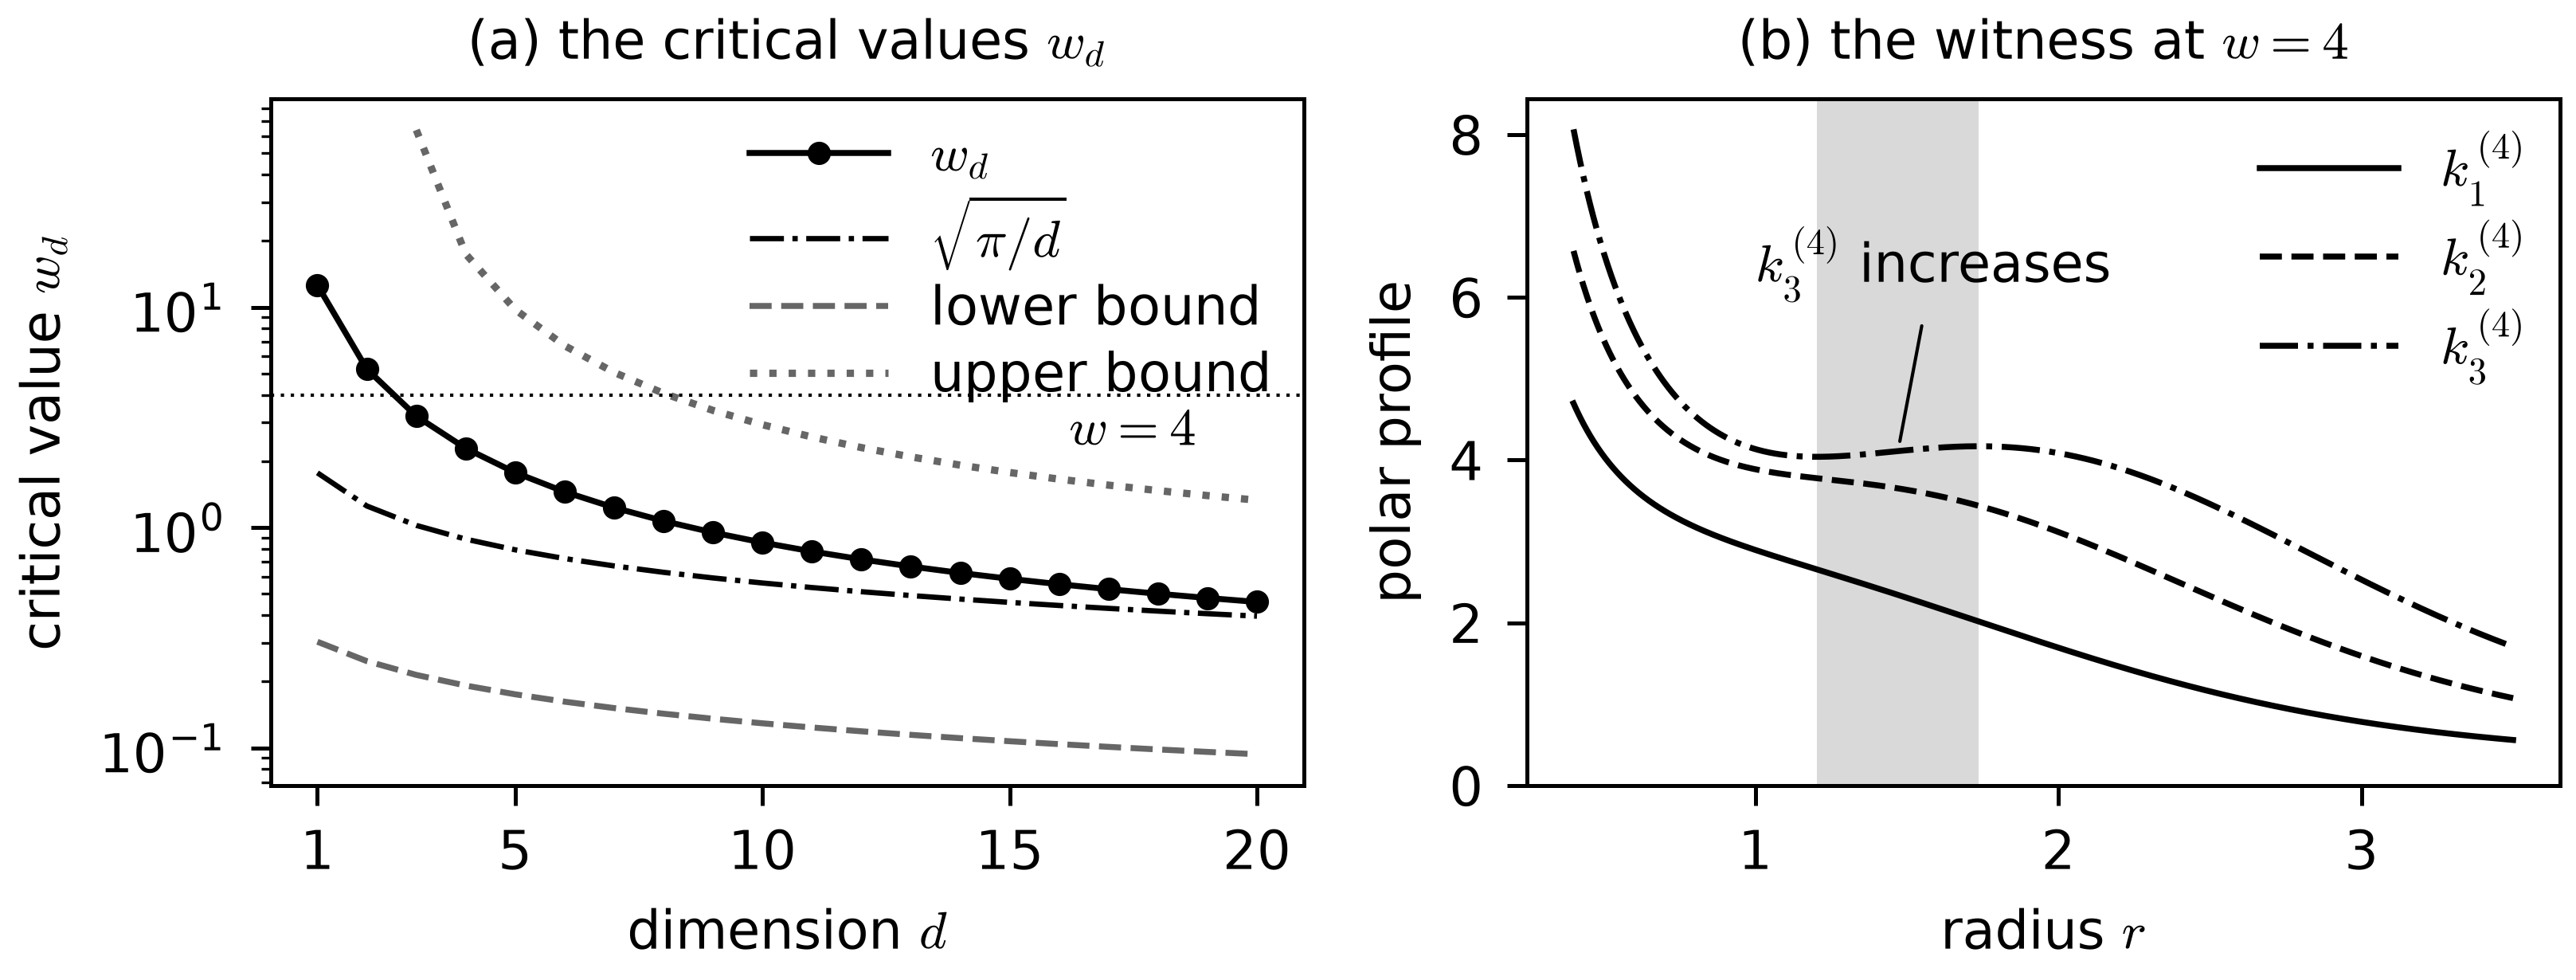
\includegraphics[width=0.86\textwidth]{fig-thresholds.png}
\caption{(a) The critical values $w_d$ of Definition~\ref{def:filtration-thresholds} for
$d = 1, \dots, 20$, computed numerically, on a logarithmic scale, with the lower and the upper
bound displayed in the text, the upper one for $d \ge 3$, and the asymptote $\sqrt{\pi/d}$ of
Theorem~\ref{thm:separating-family-critical-values}(3). The horizontal line $w = 4$ crosses the
sequence between $d = 2$ and $d = 3$. (b) The polar profiles $k^{(4)}_d$ of $F^{(4)}$
(Definition~\ref{def:filtration-thresholds}) in dimensions $1$, $2$ and $3$: nonincreasing in
dimensions $1$ and $2$, increasing on the marked interval, about $(1.20, 1.74)$, in dimension
$3$. Computed by a script deposited with the paper.}
\label{fig:thresholds}
\end{figure}

As laws the members of the family are ordinary kernels in every dimension. For every $w > 0$ and
every $D$ the function $e^{-F^{(w)}(|\xi|)}$ is the transform of a Gaussian variance mixture on
$\RR^D$, a rotation-invariant infinitely divisible law
(Proposition~\ref{prop:separating-family-mixtures}(2)). In the dimensions that do not admit
$F^{(w)}$ that law lacks self-decomposability alone, the property that gives a cascade its
stages (its clause (3)). So the family separates a kernel in every dimension from a cascade in
every dimension. Its delay profile is not monotone, and its delay exponent $F^{(w)}_{\mathrm I}$
is not causally admissible: otherwise $F^{(w)}$ would be a member of $\mathcal{S}$, and so of
every $\mathcal{A}_D$ (Proposition~\ref{prop:line-filtration}(2)).

\begin{remark}[relation to the line]\label{rem:isotropic-line}
At $d = 1$ the definitions, the classification and the threshold of this section are those of the
line. $\Orth(1) = \{\pm1\}$, so Definition~\ref{def:isotropic-operator-family} is
Definition~\ref{def:line-family}, Corollary~\ref{cor:isotropic-classification-operators} is
Theorem~\ref{thm:line-classification}, and $\mathcal{A}_1$ is the admissible cone. The polar
profile $k_1$ is the folded profile of \ref{eq:admissible-line}, so $k_1(0{+})$ is the constant
$c$ of Corollary~\ref{cor:line-threshold}, whose two regimes and threshold are
Theorem~\ref{thm:origin-boundedness-d}(2), (4) and (5). What of the line theory is not carried to
$\RR^d$ is said in \S\ref{sec:conclusion}.
\end{remark}
